\section{Performance des moteurs à gaz}

	\subsection{Intérêt de l’utilisation de l’air}

		L’utilisation de l’air comme fluide moteur, plutôt que la vapeur, apporte plusieurs avantages.

		\begin{itemize}
			\item D’une part, il est possible de se dispenser entièrement des condenseurs et refroidisseurs. La phase de refroidissement (\S\ref{ch_principe_fonctionnement_moteur} \& \S\ref{ch_demo_second_principe}) a lieu directement dans l’atmosphère, qui accueille aisément tous les gaz chauds que l’on rejette, et où l’air frais abonde\footnote{Il nous faudra toutefois bien reconnaître que ce ne sera pas nécessairement toujours le cas…}.

			À puissance égale, la masse, le volume et souvent le coût des moteurs à gaz sont donc très fortement réduits par rapport à leurs homologues à vapeur. Ceci est particulièrement intéressant lorsque le moteur doit participer à la portée de son propre poids.

			\item D’autre part, l’apport de chaleur se fait sans perte. En effet, il est possible d’ef\-fec\-tuer une combustion \emph{directement à l’intérieur} du fluide de travail --\ c’est ce que l’on nomme la combustion interne. 

			Alors que les installations à vapeur laissent s’échapper de grandes quantités de chaleur au-dessus de la chaudière (\S\ref{ch_chaudière}), les moteurs à air perdent très peu de chaleur dans les phases de combustion.

		\end{itemize}

		La combustion interne impose cependant une qualité de carburant élevée. Il n’est pas question ici d’utiliser des déchets, du bois, ou même du charbon comme combustible --\ les résidus de combustion doivent en effet circuler à l’intérieur même de la partie thermodynamique de la machine.

		Au final, la légèreté relative des moteurs à air par rapport à leurs homologues à vapeur font qu’ils sont systématiquement utilisés dans les transports où la masse joue un rôle important, tels que l’aviation ou les transports routiers.



	\subsection[Importance relative du rendement]{De l’importance relative du rendement thermodynamique}

		Nous nous risquerons à rappeler du \coursneuf que le rendement thermodynamique ne dicte pas seul le choix des cycles thermodynamiques. Il nous faut toujours tenir compte du coût économique marginal du travail produit (c’est-à-dire la facilité technologique de fonctionnement de la machine) et du coût initial d’investissement.

		Nous ferons ainsi le pari que lors de l’acquisition de son premier véhicule, l’étu\-diant/e favorisera le coût d’achat à la consommation de carburant --\ de même qu’il/\-elle n’optera pas pour une motorisation de compétition nécessitant une maintenance incessante.



	\subsection{Le rapport des puissances}
	\label{ch_rapport_des_puissances}

		Lorsque les compressions et détentes ne sont pas réversibles, le rendement d’un moteur descend en dessous de celui d’un moteur de Carnot fonctionnant entre les mêmes températures\footnote{Rappelons que le rendement de ce moteur idéal est \textit{déjà très bas} : voir le \courssept.}. Ces irréversibilités peuvent même réduire le rendement à zéro, le moteur tournant alors sans produire de travail utile (exactement comme un moteur automobile débrayé).

		Dans de nombreux moteurs, l’efficacité des composants varie fortement avec la vitesse de fonctionnement. Ainsi, il est important de connaître le comportement du moteur lorsque ses composants fonctionnent hors de leurs conditions optimales. Le rapport des puissances est un concept qui permet de quantifier cela --\ la «~robustesse~» du cycle thermodynamique, en quelque sorte.

		Pour l’aborder, étudions le cas d’une machine dont la compression et la détente sont réversibles. Les puissances en jeu sont comme décrites en \cref{fig_rapport_puissances_1}.

		\begin{figure}
			\begin{center}
				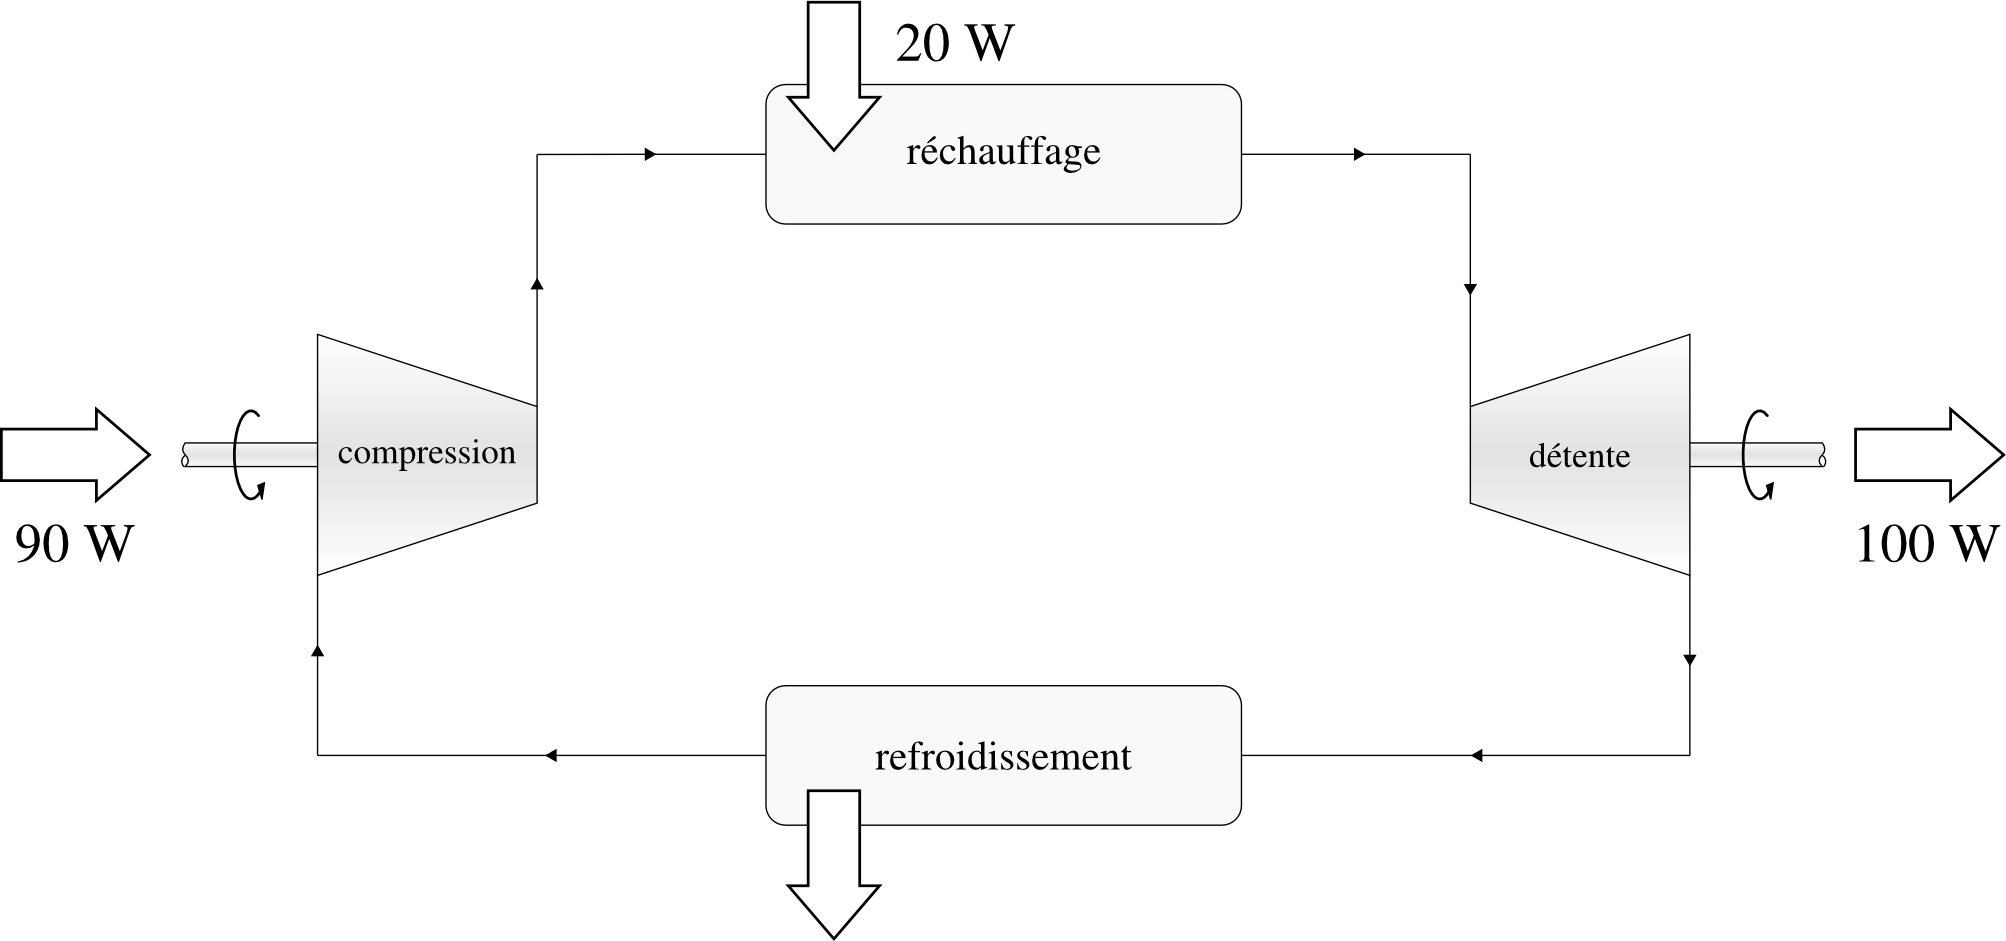
\includegraphics[width=\textwidth]{images/cours10-img3.png}
			\end{center}
			\caption{Cycle idéal d’une machine à faible rapport de puissances.}
			\label{fig_rapport_puissances_1}
		\end{figure}

		Si maintenant la turbine se voyait soudainement affublée d’un rendement isentropique de~\SI{95}{\percent}, elle ne fournirait plus que \SI{95}{\watt}. La puissance effective du moteur passerait alors de~\num{10}~à~\SI{5}{\watt} --\ une réduction de~\SI{50}{\percent}.

		Comparons maintenant ce cas avec un cycle de même rendement, même puissance, mais dont les puissances n’ont pas le même rapport, comme en \cref{fig_rapport_puissances_2}.

		\begin{figure}
			\begin{center}
				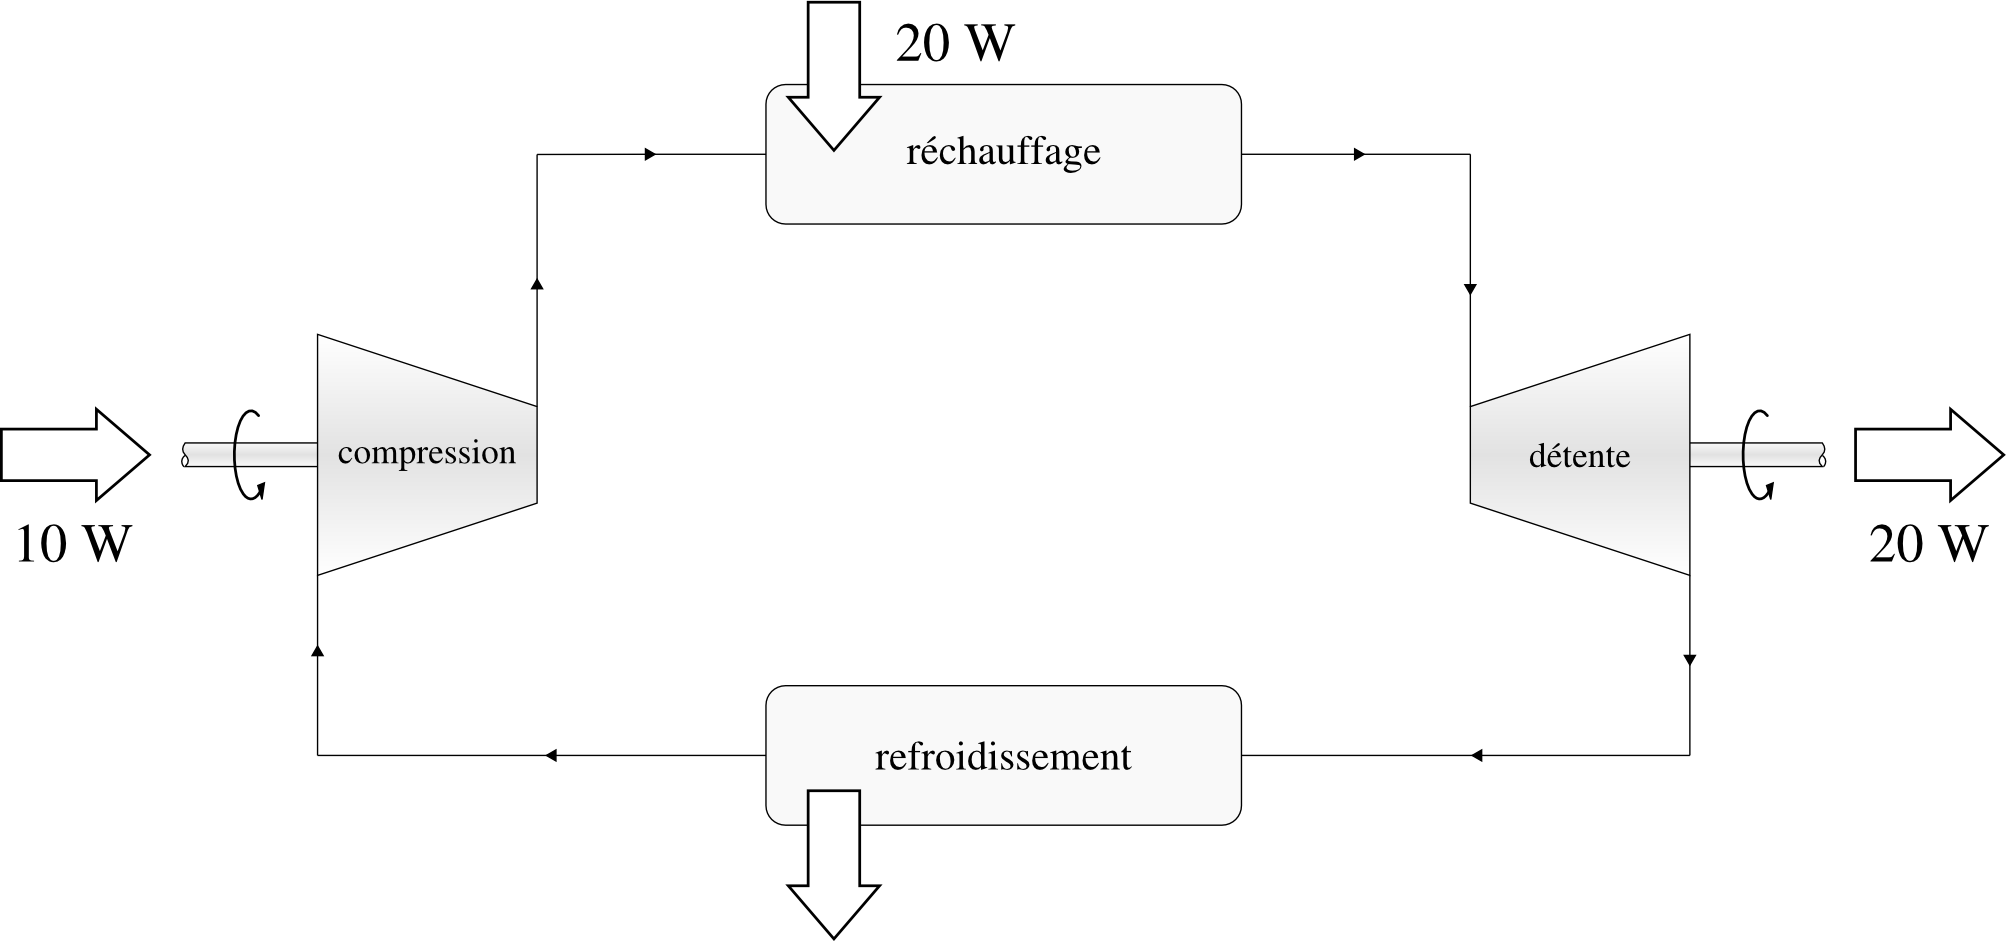
\includegraphics[width=\textwidth]{images/cours10-img4.png}
			\end{center}
			\caption{Cycle idéal d’une machine à fort rapport de puissances.}
			\label{fig_rapport_puissances_2}
		\end{figure}

		Le cycle a le même rendement global, mais le rapport entre la puissance de la turbine et celle que fournit la machine est beaucoup plus grand. Si l’efficacité isentropique de la turbine passait de~\SI{100}{\percent} à~\SI{95}{\percent}, la puissance effective du moteur passerait de~10~à~\SI{9}{\watt} --\ une baisse de~\SI{10}{\percent} seulement.

		On peut ainsi voir l’intérêt d’une machine dont ce rapport est grand. Lorsque l’ef\-fi\-ca\-ci\-té des turbines et compresseurs est réduite (par exemple parce qu’ils ne fonctionnent pas à vitesse optimale), sa puissance et son efficacité baissent beaucoup moins vite que celles d’une machine dont le rapport est plus faible\footnote{On peut faire l’analogie avec la notion de \emph{marge} en économie, qui est un paramètre tout aussi important que le bénéfice pour mesurer la viabilité financière d’une organisation.}\nolinebreak.

		On définit formellement le \vocab{rapport des puissances} (en anglais : \vocabe{work ratio}) d’un moteur comme le rapport entre sa puissance nette et sa puissance brute :

		\begin{IEEEeqnarray}{rCl}
			r_\text{w} 	& \equiv	& 	\frac{\dot{W}_\text{net}}{\dot{W}_\text{brut}}		\label{eq_rapport_puissances}\\
			r_\text{w} 	& = & 		\frac{\dot{W}_\text{détente} + \dot{W}_\text{compression}}{\dot{W}_\text{détente}}
		\end{IEEEeqnarray}

		\begin{equationterms}
			\item où \tab $r_\text{w}$ \tab est le rapport des puissances (sans unité) ;
			\item \tab $\dot{W}_\text{détente}$ \tab est la puissance fournie pendant les détentes (ex. par la turbine) ;
			\item et \tab $\dot{W}_\text{compression}$ \tab la puissance consommée lors des compressions (ex. par le compresseur ou la pompe).
		\end{equationterms}

		Le moteur de Carnot est l’exemple-type d’un cycle thermodynamique à haut rendement mais dont le rapport des puissances est très faible. En traçant le cycle sur un diagramme pression-volume (\cref{fig_p-v_gp_carnot}) cette faiblesse ressort bien : les courbes lors des phases de compression et détente sont très proches l’une de l’autre. Rankine, lorsqu’il modifie ce cycle (\S\ref{ch_cycle_de_rankine}), augmente considérablement le rapport des puissances.

		D’une façon générale, une grande efficacité thermodynamique globale requiert un grand taux de compression (afin d’obtenir une haute température avant que le transfert de chaleur ne soit initié). Un grand rapport de puissances requiert un faible travail de compression (afin de minimiser la sensibilité du moteur aux irréversibilités).

		Ces deux objectifs sont donc souvent contradictoires et il redviendra à l’ingénieur/e thermodynamicien/ne de concevoir un cycle avec ces deux paramètres en tête.

		 

	\subsection{Masse et encombrement}

		Le contexte dans lequel le moteur est utilisé impose souvent de sacrifier son efficacité au profit d’autres caractéristiques.

		Ainsi, sur un moteur aéronautique, une augmentation du rendement n’est pas toujours justifiée si elle provoque une augmentation du poids ou de l’encombrement. Un aéronef plus lourd doit fournir une plus grande portance, ce qui augmente la traînée… et donc la demande en énergie.

		Les constructeurs aéronautiques utilisent les concepts de \vocab{poussée et puissance spécifiques}, $\frac{P}{\dot m}$ et $w_\text{net}$, c’est-à-dire la poussée et la puissance du moteur divisées par le débit d’air qui le traverse, pour comparer sommairement les moteurs entre eux. Un moteur avec un grand rapport puissance/poids est souvent caractérisé par une grande puissance spécifique.



\section{Motorisations à pistons}



	\subsection{Intérêt des moteurs à pistons}

		Les moteurs à mouvement alternatif (souvent dits «~à pistons/cylindres~») ne fonctionnent pas en régime continu. Ils admettent une quantité d’air finie, et le cycle moteur est effectué sur cette masse. Le cycle est répété plusieurs fois dans le temps pour fournir une puissance continue (un moteur automobile effectue usuellement une cinquantaine de cycles par seconde).

		Le principal avantage de ces moteurs est que d’un point de vue thermodynamique, la manipulation d’une masse fixe d’air est beaucoup plus aisée que celle d’un flux continu. Il est possible, par exemple, d’effectuer une combustion à température constante (tel que le préconise Carnot) en faisant varier le volume pendant la combustion. La même opération en régime continu requerrait que la combustion s’ef\-fec\-tue au sein d’une turbine, ce que l’on ne sait encore pas faire à l’échelle industrielle.

		Ainsi, à taux de compression égal, un compresseur de turboréacteur requiert une vitesse élevée et une géométrie très complexe, tandis qu’un moteur à mouvement alternatif ne requiert qu’un simple piston dans un cylindre.

		Un second avantage des moteurs à pistons est que la température maximale du cycle n’y est atteinte que sporadiquement (périodiquement, mais toujours brièvement). Il est ainsi possible, lors de la combustion, de faire atteindre au gaz des températures qui dépassent les limites métallurgiques du moteur, avec les avantages pour le rendement que nous avons abordés au \courssept.

		Le poids de ses mécanismes (bielles, vilebrequin, soupapes, circuits divers), en revanche, défavorise le moteur à pistons lorsque de très grandes puissances et vitesses de rotation sont requises.



	\subsection{Le cycle d’Otto}

		On doit à l’allemand \wf{Nikolaus Otto}, en 1876, la mise au point du moteur que l’on connaît aujourd’hui sous le nom de «~\vocab{moteur à essence}~». Le cycle de ce moteur, appellé \vocab{cycle d’Otto}, est décrit en \cref{fig_cycle_otto}. En théorie, les échanges de chaleur se font à volume constant et la compression et la détente sont isentropiques.

		\begin{figure}
			\begin{center}
				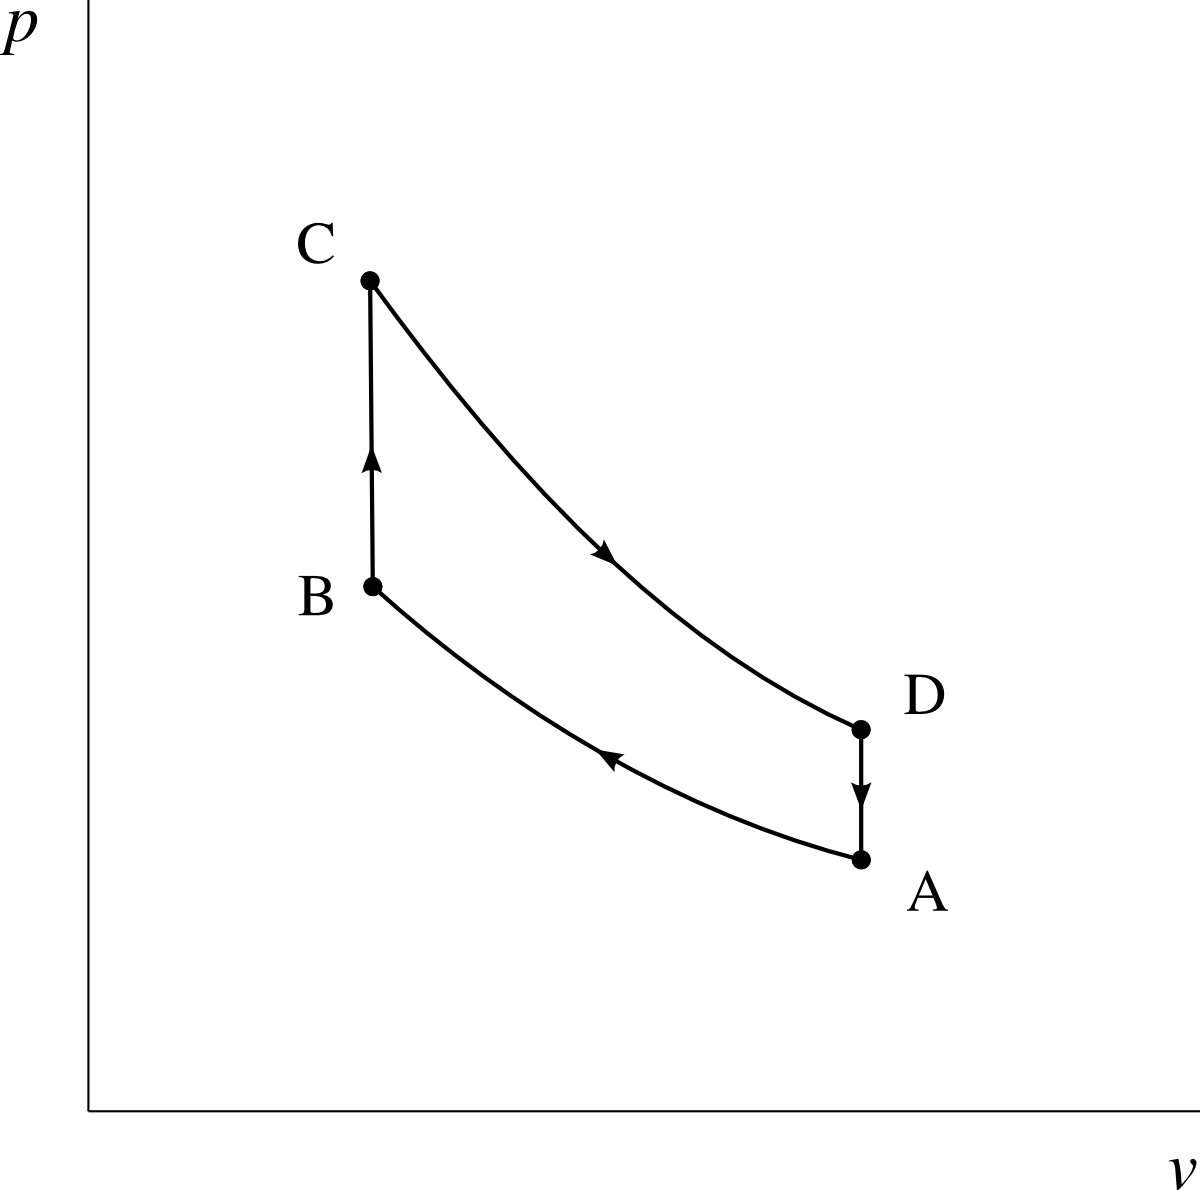
\includegraphics[width=6cm]{images/pv_gp_otto.png}
				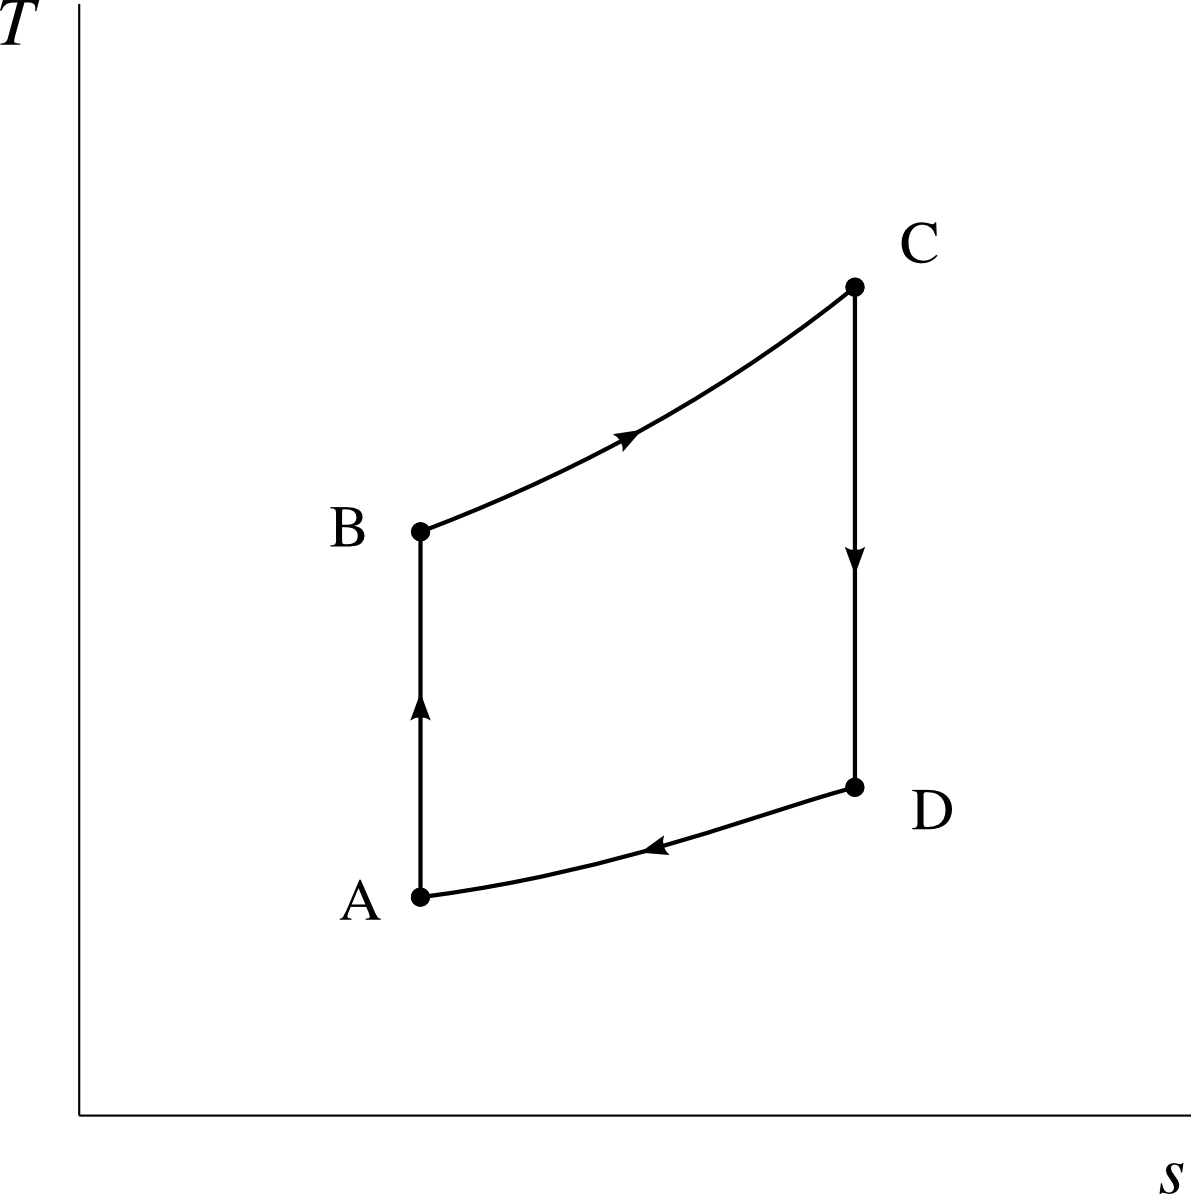
\includegraphics[width=6cm]{images/ts_gp_otto.png}
			\end{center}
			\caption{Cycle théorique d’Otto (diagrammes pression-volume et température-entropie).
			Ces graphiques représentent le trajet idéal, sans irréversibilité de compression ou détente.}
			\label{fig_cycle_otto}
		\end{figure}

		Le rendement du cycle d’Otto théorique est calculable sans grande difficulté.

		La chaleur est reçue par l’air à volume constant :
		\begin{equation}
			q_\text{combustion} = c_v (T_\C - T_\B )
		\end{equation}

		Le rejet de chaleur est effectué à volume constant%
			\footnote{Le refroidissement, en pratique, est effectué hors du moteur (à la sortie du pot d’échappement). D’un point de vue thermodynamique, l’air poursuit son cycle dans l’atmosphère avant de pénétrer à nouveau dans le moteur.}
		(hors du moteur) :
		\begin{equation}
			q_{\text{refroidissement}} = c_v (T_\A - T_\D)
		\end{equation}

		Ainsi, puisqu’en théorie aucun transfert de chaleur n’a lieu dans les phases de compression et détente, et si l’on considère que les propriétés ($c_v$) du gaz ne changent pas pendant la combustion, avec l’\cref{def_rendement_moteur} le rendement $\eta_{Otto}$ du cycle théorique est simplement :
		\begin{equation*}
			\eta_{Otto} = \left| \frac{q_\text{comb.} + q_\text{refr.}}{q_\text{comb.}} \right| = 1 + \frac{q_\text{refr.}}{q_\text{comb.}} = 1 + \left( \frac{T_\A - T_\D}{T_\C - T_\B } \right)
		\end{equation*}

		En définissant le taux de compression $r_v$ comme :
		\begin{equation}
			r_v \equiv  \frac{v_\A}{v_\B }
		\end{equation}

		il est possible de montrer que le rendement s’exprime seulement selon

		\begin{equation}
			\eta_\text{Otto} = 1 - \frac{1}{r_v^{\gamma -1}}
		\end{equation}

		On constate ainsi que le rendement du moteur d’Otto dépend uniquement du taux de compression --\ et non de la quantité de chaleur apportée pendant la combustion\footnote{L’étudiant/e n’aura pas tort de se surprendre de ce résultat --\ la température maximale du cycle n’a pas d’influence sur le rendement ! Dans ce cycle, l’augmentation de la température moyenne d’apport de chaleur est exactement compensée par l’augmentation de la température moyenne de refroidissement.}\nolinebreak.
		Toutefois, cette équation n’est valide qu’en négligeant le changement des propriétés de l’air pendant la combustion, ainsi que les irréversibilités lors de la compression et de la détente. Il ne faut donc l’interpréter qu’avec la plus grande prudence.

		Pour augmenter l’efficacité de leurs moteurs, les motoristes cherchent perpétuellement à en augmenter le taux de compression. Une limite immédiate à ce taux est la température à laquelle le mélange air-carburant s’enflamme spontanément, provoquant une combustion prématurée.



	\subsection{Le cycle de Diesel}

		Fruit du travail patient et soigneux de son inventeur, \wf{Rudolf Diesel}, le \vocab{moteur Diesel} propulse aujourd’hui l’écrasante majorité des transports commerciaux sur route et sur mer.

		Le cycle Diesel diffère de celui d’Otto par le fait que l’apport de chaleur se fait à pression constante et non à volume constant (\cref{fig_cycle_diesel}).

		\begin{figure}
			\begin{center}
				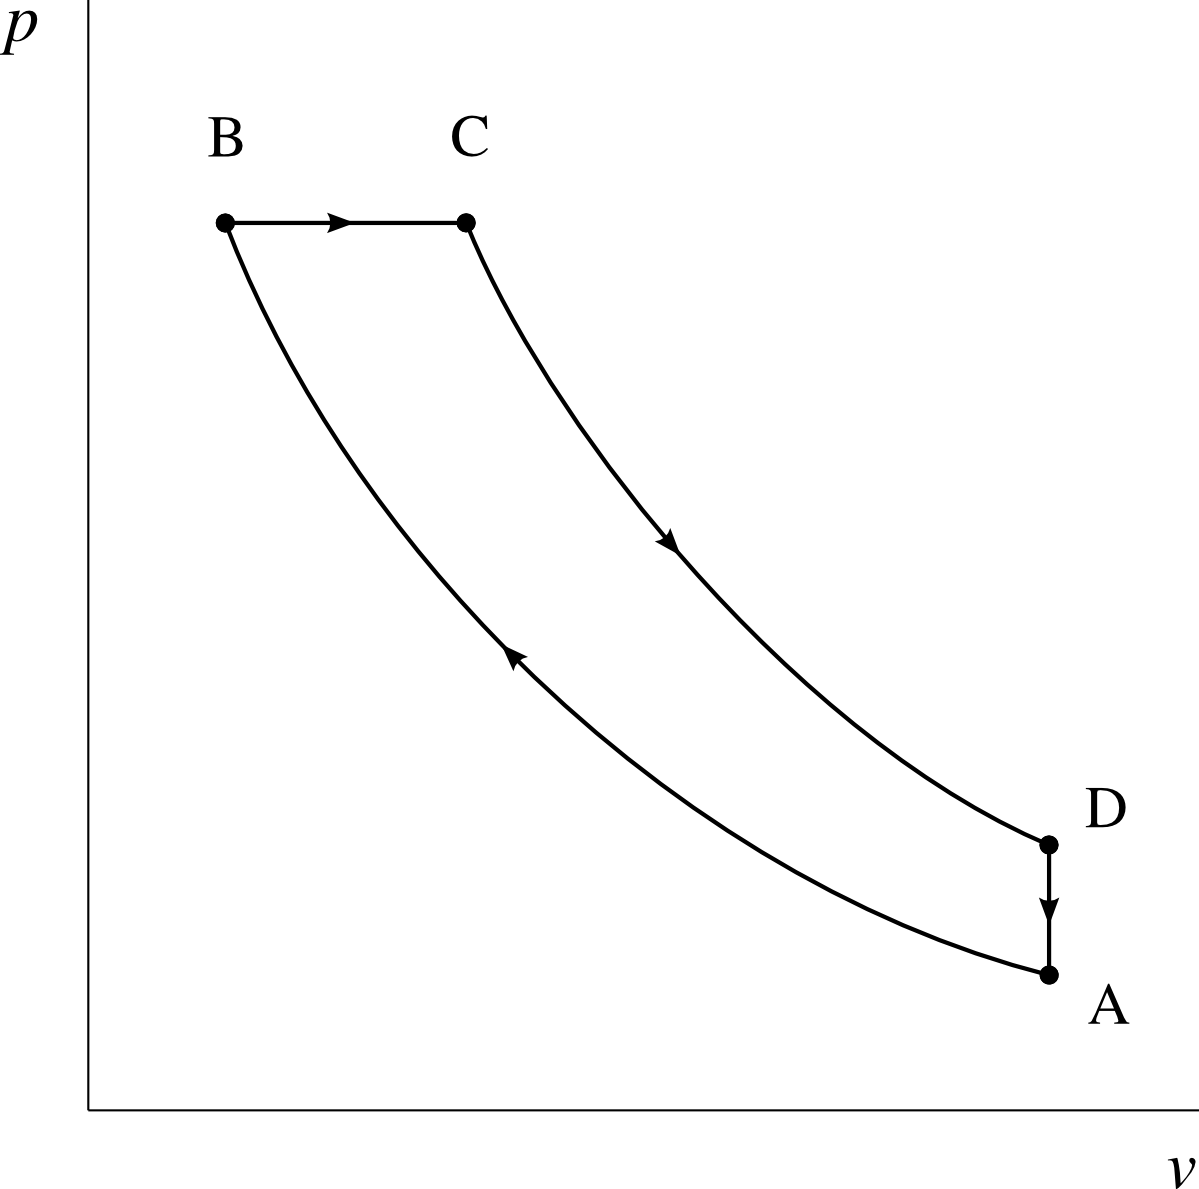
\includegraphics[width=6cm]{images/pv_gp_diesel.png}
				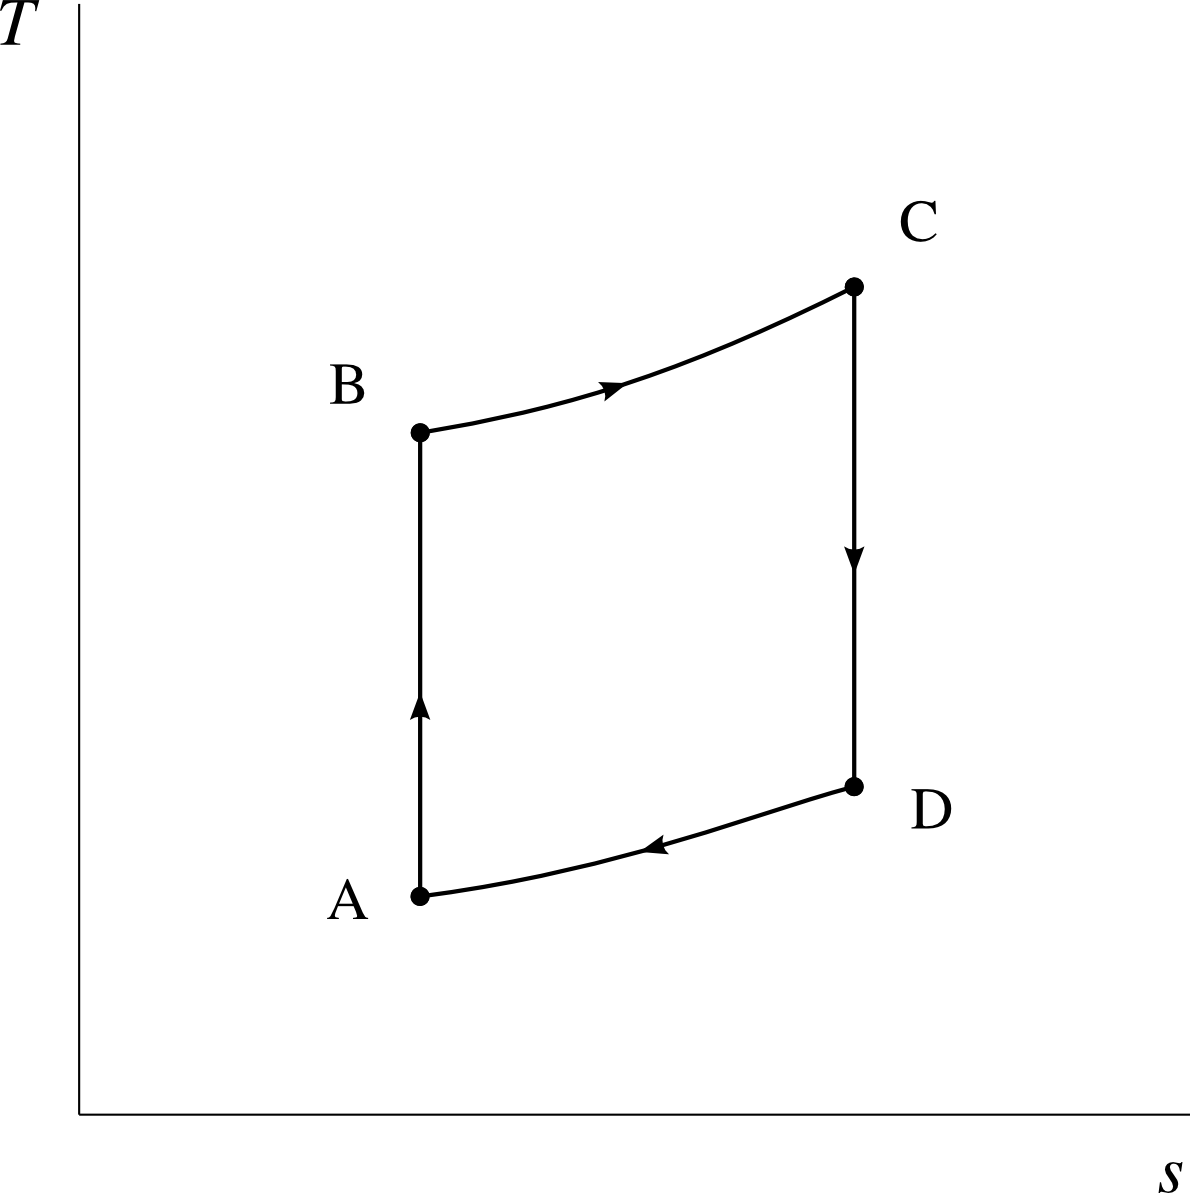
\includegraphics[width=6cm]{images/ts_gp_diesel.png}
			\end{center}
			\caption{Cycle théorique de Diesel (diagrammes pression-volume et température-entropie).
			Ces graphiques représentent le trajet idéal, sans irréversibilité de compression ou détente.}
			\label{fig_cycle_diesel}
		\end{figure}

		La chaleur fournie au gaz s’exprime cette fois selon :
		\begin{equation}
			q_\text{combustion} = c_p (T_\C - T_\B )
		\end{equation}

		et du travail est fourni pendant cet apport de chaleur.

		Il n’existe pas d’expression simple pour le rendement, qui ne dépend plus uniquement du taux de compression -- il faudra le calculer en étudiant le cycle pas à pas (\ref{def_rendement_moteur}).

		À taux de compression égal (c’est-à-dire pour un piston-cylindre de géométrie donnée), le cycle Diesel a un rendement plus faible que celui d’Otto. Ce n’est bien sûr pas une comparaison utile pour comprendre le moteur de Rudolf Diesel, qui s’intéressait à deux possibilités :

		\begin{itemize}
			\item augmenter le taux de compression (pour cela, il lui fallait attendre la fin de la compression pour injecter le carburant, afin d’éviter un allumage prématuré),
			\item et apporter la chaleur à une température moyenne plus grande\footnote{La publication fascinante de Diesel en 1893, \textit{Theorie und Construktion eines rationnellen Wärmemotors zum Ersatz der Dampfmaschinen und der bis heute bekannten Verbrennungsmotoren}, est sans équivoque : le but est d’imiter au plus près le cycle décrit par Carnot.}\nolinebreak.
		\end{itemize}

		La pression maximale que peut soutenir le moteur est donc atteinte dès la fin de la compression, et la combustion se fait ainsi, en théorie, à pression constante.

		Une particularité du fonctionnement du moteur Diesel est que la masse d’air admise dans le cylindre ne dépend pas de la puissance demandée (elle est constante à chaque cycle --\ seule la quantité de carburant injectée est variée). L’efficacité du cycle, contrairement à celui d’Otto, est peu affectée lorsque le moteur fonctionne en charge partielle.

		Notons que d’un point de vue thermodynamique, le carburant utilisé n’a pas d’im\-por\-tan\-ce. Par exemple, Rudolf Diesel travaillait initialement avec de la poudre de charbon, et les moteurs Diesel maritimes fonctionnent avec des produits proches du pétrole brut.



	\subsection{Cycles thermodynamiques réels}

		L’étude des cycles moteurs réels peut faire l’objet de toute une année d’études. Nous nous contenterons de remarquer que les cycles décrits plus haut ne sont que des cycles idéaux --\ ils servent principalement d’étalons pour comparer les moteurs réels entre eux.

		Tout d’abord, l’adoption de l’injection de carburant contrôlée par électronique dans les moteurs a considérablement réduit la différence entre les cycles des moteurs dits «~essence~» et «~Diesel~», en permettant un très bon contrôle de la pression et de la température pendant les phases de combustion.

		En pratique, de nombreux autres facteurs éloignent les cycles réels des cycles théoriques que nous avons dessinés (\cref{fig_cycle_otto_réel}), parmi lesquels :

		\begin{itemize}
			\item La nécessité de vidanger l’air et les produits de combustion à l’intérieur du cylindre après le cycle, et l’impossibilité de le faire complètement ;
			\item Le fait que le volume occupable par le gaz soit lié à la rotation du moteur,\footnote{Dans tous les moteurs usuels, le piston est lié à l’axe de transmission par l’intermédiaire d’une bielle et d’un vilebrequin. Impossible alors d’effectuer une combustion à volume constant sans arrêter le moteur…}
			et donc qu’il n’est pas possible de le contrôler indépendamment de la vitesse du moteur ;
			\item Les irréversibilités lors des compressions et détentes causées par les mouvements rapides des pistons ;
			\item Les transferts de chaleur vers et depuis les cylindres pendant le cycle ;
			\item Les fuites des gaz dans les interstices entre pistons et cylindres.
		\end{itemize}

		\begin{figure}
			\begin{center}
				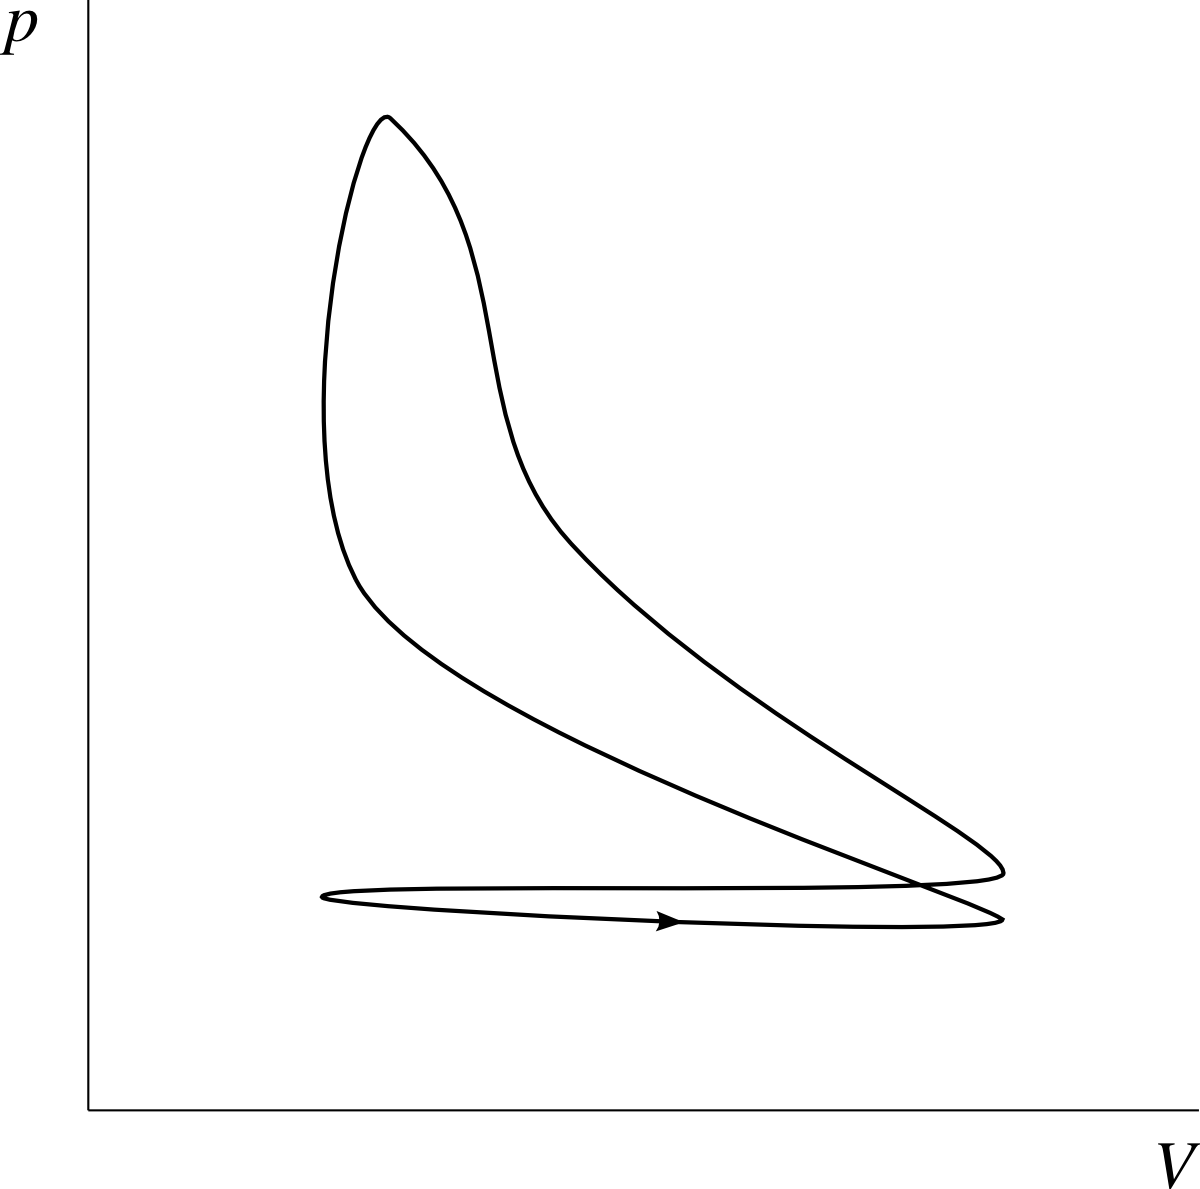
\includegraphics[width=9.5cm]{images/pv_moteur_reel.png}
			\end{center}
			\caption{Évolution réaliste de la pression et du volume pendant un cycle dans un moteur essence.}
			\label{fig_cycle_otto_réel}
		\end{figure}

		Bien sûr, comme pour tout autre moteur, de nombreux autres facteurs sont à prendre en compte pendant la mise au point d’un cycle thermodynamique, parmi lesquels le poids et la taille des mécanismes entourant la chambre de combustion, le comportement du moteur à différents régimes, et ses émissions dans l’atmosphère.


 

\section{Composants des turbomachines}

	Avant de nous plonger dans les cycles des moteurs à turbines, nous nous proposons de rappeler brièvement le fonctionnement des composants principaux. Comme les turbomachines fonctionnent en régime permanent, nous ferons à partir d’ici systématiquement appel aux notions du \courstrois.

	Pour les raisons évoquées en \S\ref{ch_expressions_puissances_vapeur}, les transferts de travail et de chaleur sont espacés physiquement dans le moteur.



	\subsection{Compresseur}

		Les phases de compression et de détente dans les moteurs se font très souvent de façon adiabatique et toujours de façon irréversible. L’écoulement des fluides au sein du compresseur des moteurs modernes est extrêmement complexe et la compression y est difficile à effectuer\footnote{Au sein d’un bon cours de mécanique des fluides, l’étudiant/e aura l’occasion de découvrir que le gradient de pression au sein d’un compresseur favorise la séparation de la \vocab{couche limite}. Ainsi, on utilise toujours un plus grand nombre d’étages dans un compresseur que dans turbine de même puissance, où le gradient est favorable.}\nolinebreak.
		C’est un composant lourd, volumineux, et dont la géométrie est complexe (figures~\ref{fig_schéma_compresseur1} et~\ref{fig_schéma_compresseur2})

		\begin{figure}
			\begin{center}
				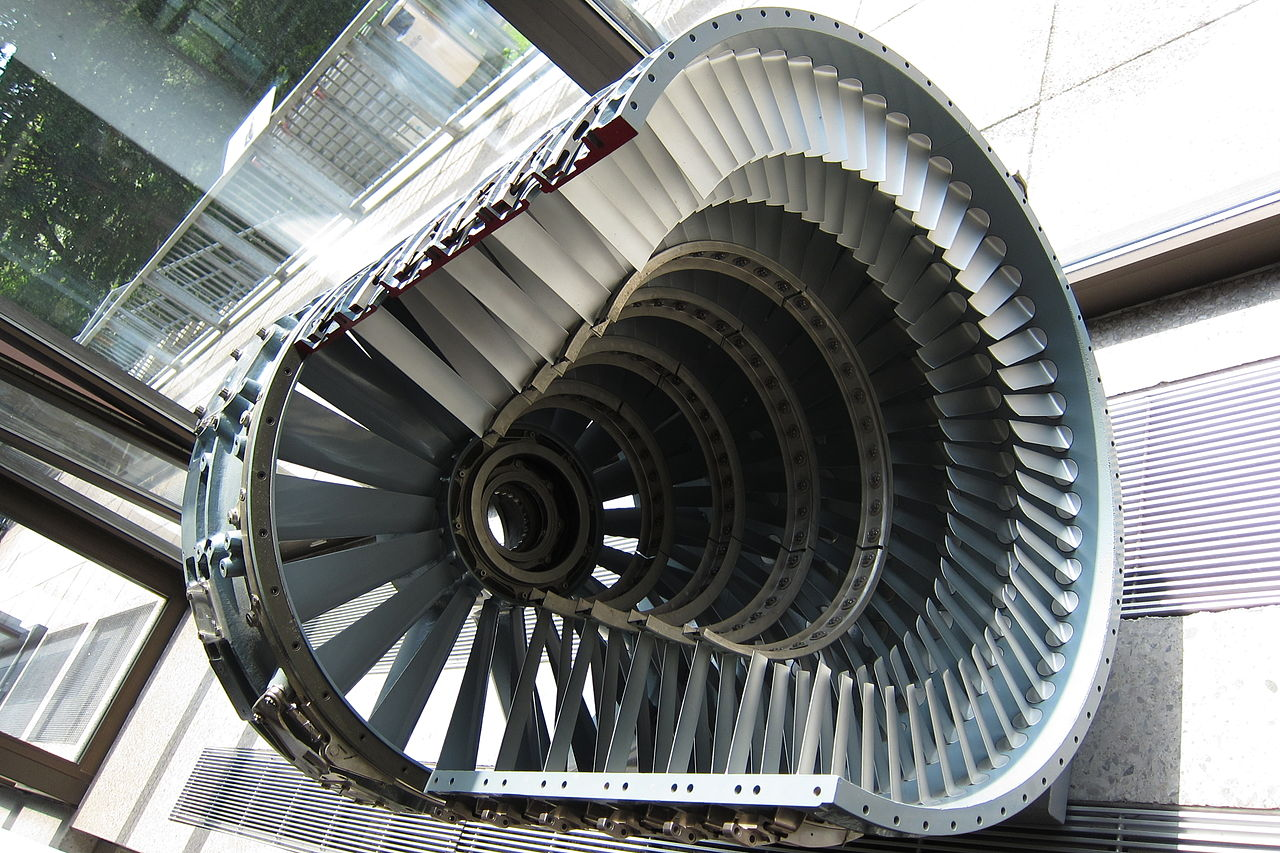
\includegraphics[width=8cm]{images/photo_compresseur.jpg}
			\end{center}
			\supercaption{Caisson de stators accueillant le compresseur axial d’un turboréacteur.}{\wcfile{Compressor_case_from_turbofan.jpg}{Photo} \ccbysa \olivier}
			\label{fig_schéma_compresseur1}
		\end{figure}

		\begin{figure}
			\begin{center}
				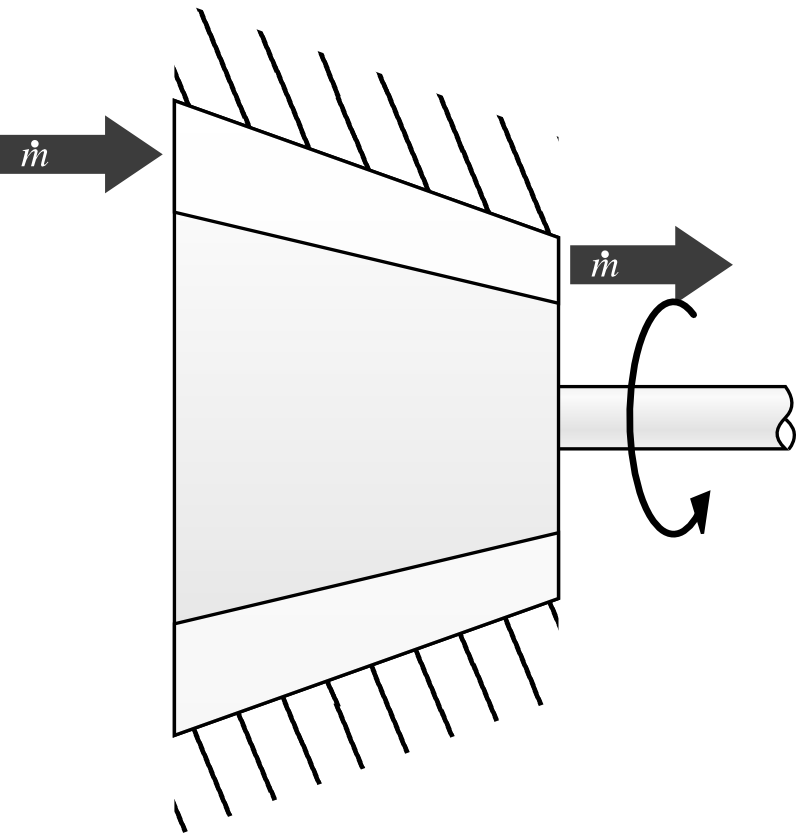
\includegraphics[width=4cm]{images/symbole_compresseur.png}
			\end{center}
			\supercaption{Représentation schématique d’un compresseur à air.}{}
			\label{fig_schéma_compresseur2}
		\end{figure}

		Pour quantifier l’efficacité de la phase de compression, on utilise le concept de l’\vocab{efficacité isentropique} $\eta_\C$, comme pour la turbine (\ref{def_efficacité_isentropique_turbine}). Nous comparons ainsi la puissance minimale, consommée dans le cas théorique isentropique, avec la puissance consommée en réalité :
		\begin{equation}
			\eta_\C \equiv  \frac{\dot{W}_\text{Compresseur isentropique}}{\dot{W}_\text{Compresseur réel}}
			\label{def_efficacité_isentropique_compresseur}
		\end{equation}

		\begin{equationterms}
			\item pour un compresseur ;
			\item où \tab $\dot{W}_\text{Compresseur réel}$ \tab\tab\tab est la puissance réelle consommée par le compresseur,
			\item et \tab $\dot{W}_\text{Compresseur isentropique}$ \tab la puissance d’un compresseur isentropique qui fonctionnerait avec le même débit de masse, entre les deux mêmes pressions.
		\end{equationterms}

		Comme celle d’une turbine, l’efficacité isentropique d’un compresseur est toujours inférieure à~1.

		En négligeant les variations de l’énergie mécanique, nous pouvons relier la puissance à la température :
		\begin{equation}
			w_\text{compresseur} = c_p (T_\text{B réel} - T_\A ) = \frac{c_p (T_\text{B is.} - T_\A )}{\eta_\C}
			\label{eq_puissance_compresseur}
		\end{equation}

		\begin{equationterms}
			\item où \tab $w_\text{compresseur}$ \tab est la puissance spécifique consommée par le compresseur (\si{\joule\per\kilogram}),
			\item 	\tab $T_\text{B is.}$ \tab\tab\tab\tab est la température idéale de sortie (compresseur isentropique),
			\item et \tab $T_\text{B réel}$ \tab\tab\tab est la température à la sortie du compresseur réel.
		\end{equationterms}

		Notons qu’en pratique, de nombreux prélèvements d’air sont effectués au sein du compresseur, pour alimenter d’autres équipements et pour refroidir la turbine.



	\subsection{Chambre de combustion}

		L’apport de chaleur se fait dans une ou plusieurs chambres de combustion (figures \ref{fig_chambre_de_combustion1} et~\ref{fig_chambre_de_combustion2}). L’air y est réchauffé à pression constante par combustion ; sa température et son volume spécifique augmentent brutalement.

		\begin{figure}
			\begin{center}
				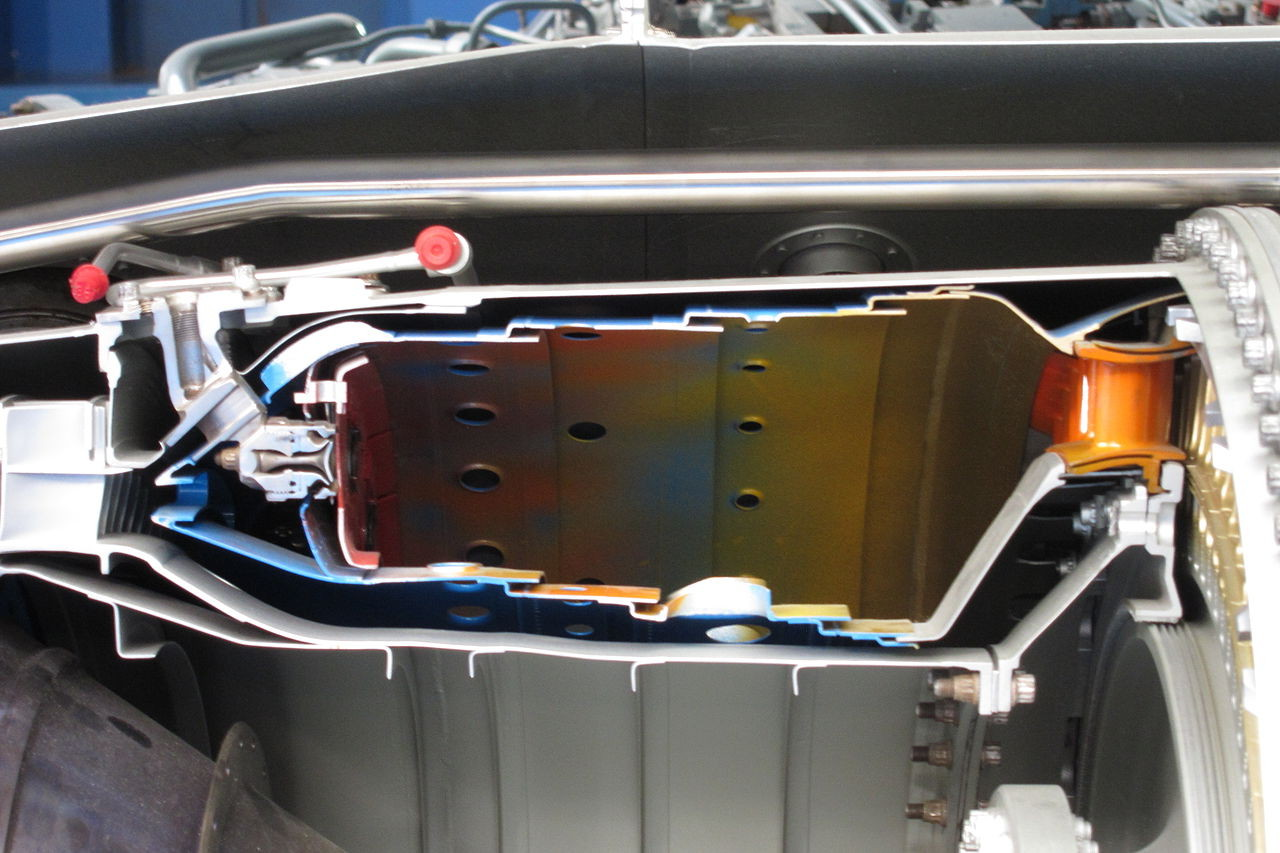
\includegraphics[width=9cm]{images/photo_chambre_combustion.jpg}
			\end{center}
			\supercaption{Section d’une chambre de combustion annulaire.\\
			La photo montre une découpe d’un petit turboréacteur (Rolls-Royce Turboméca Adour) dans lequel l’écoulement se faisait de gauche à droite.}{\wcfile{Combustor_of_sectioned_Rolls-Royce_Turboméca_Adour_turbofan.jpg}{Photo} \ccbysa \olivier}
			\label{fig_chambre_de_combustion1}
		\end{figure}

		\begin{figure}
			\begin{center}
				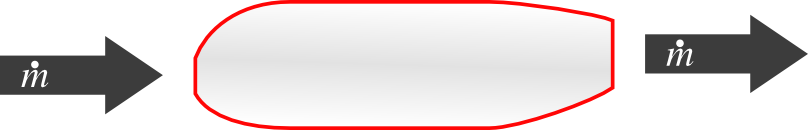
\includegraphics[width=7cm]{images/symbole_chambre_combustion.png}
			\end{center}
			\caption{Représentation schématique d’une chambre de combustion.}
			\label{fig_chambre_de_combustion2}
		\end{figure}

		Aucun travail n’est apporté, et, en théorie, la pression y reste constante.

		Comme l’apport de chaleur se fait au sein du gaz même, la température maximale du cycle n’est pas limitée par la transmission de chaleur à travers une paroi. La température maximale de l’air peut donc dépasser celle de fonte de la chambre, qui est isolée avec plusieurs couches d’air comprimé. Cela permet un gain de température par rapport aux installations à vapeur qui avoisine usuellement \SI{200}{\kelvin}.

		La puissance délivrée dans la chambre de combustion s’exprime simplement par :
		\begin{equation}
			q_{\text{chambre}} = c_p (T_\B - T_\A )
		\end{equation}

		En pratique, la chambre de combustion, siège d’écoulements très complexes,\footnote{Les écoulements au sein de la chambre de combustion dépendent de façon corrélée de la chimie de combustion, de la variation de la température, et de la vitesse des particules.}
		provoque une légère perte de pression des gaz. De plus, les propriétés de l’air changent avec la combustion --\ la valeur de $c_p$ augmente de~\SI{10}{\percent} environ.

		L’influence du débit de masse du carburant $m_{carburant}$, toujours beaucoup plus faible que celui de l’air, peut être négligée sans danger.



	\subsection{Turbine}

		Le rôle de la turbine (\cref{fig_illustration_turbine1} et~\ref{fig_illustration_turbine2}) est d’alimenter le compresseur : elle doit donc extraire de l’air une puissance suffisante pour faire fonctionner ce dernier et compenser d’éventuelles pertes de transmission (usuellement autour de~\SI{1}{\percent}). En fonction de la configuration de la turbomachine, la turbine pourra ensuite extraire encore de l’énergie, pour alimenter d’autres composants (hélice, générateur électrique,~etc.).

		\begin{figure}
			\begin{center}
				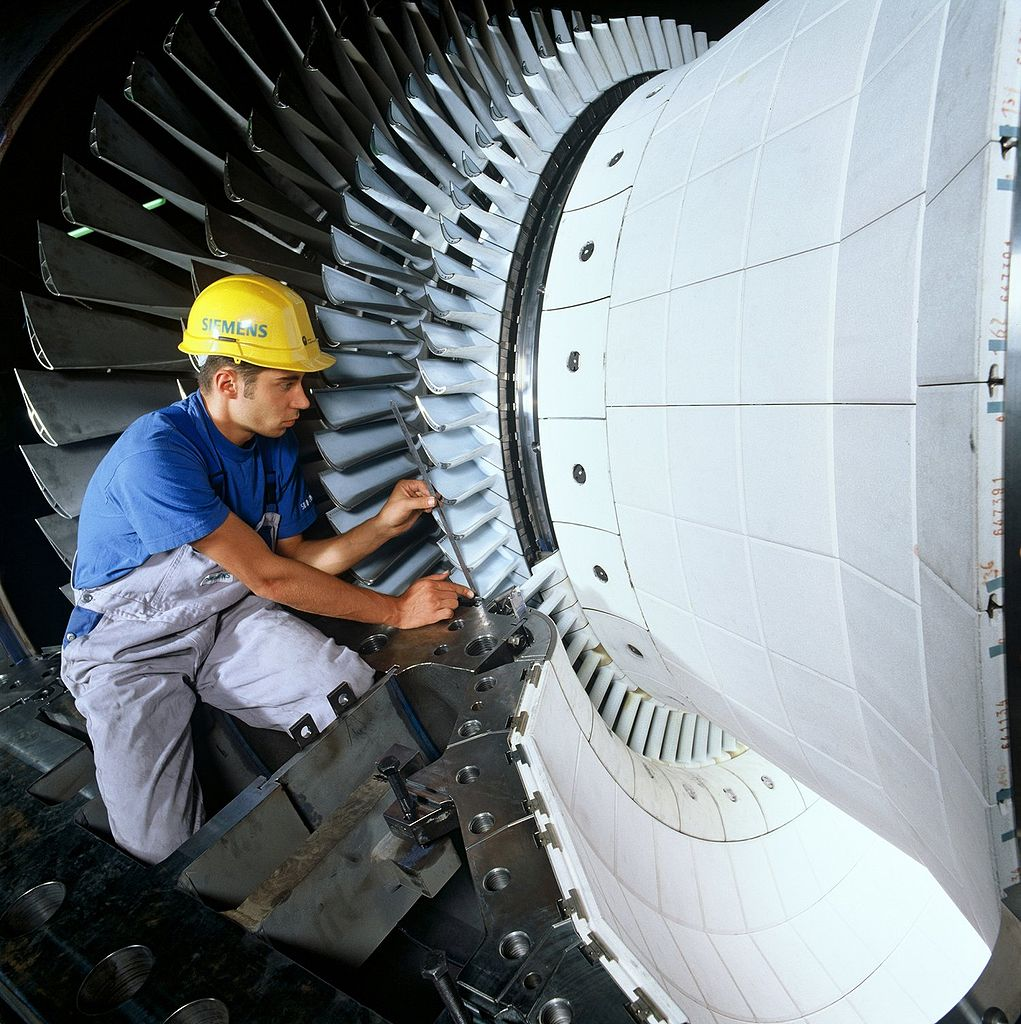
\includegraphics[width=9cm]{images/photo_turbine.jpg}\hspace{0.2cm}
			\end{center}
			\supercaption{Turbine d’un turbomoteur générateur.\\
			La turbine photographiée (Siemens SGT5) peut accepter un débit d’air et d’eau de~\SI{690}{\kilogram\per\second}. Elle transmet une puissance à l’arbre d’environ \SI{500}{\mega\watt}.}{\wcfile{Gasturbine_Montage01.jpg}{Photo} \ccbysa Siemens Pressebild}
			\label{fig_illustration_turbine1}
		\end{figure}

		\begin{figure}
			\begin{center}
				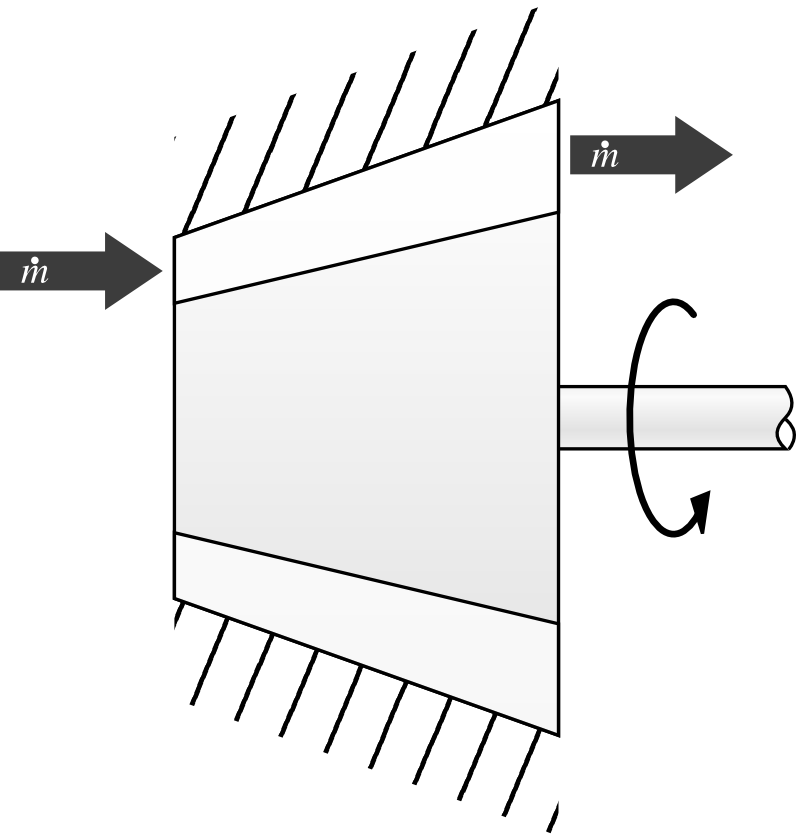
\includegraphics[width=4cm]{images/symbole_turbine.png}
			\end{center}
			\caption{Représentation schématique d’une turbine à gaz.}
			\label{fig_illustration_turbine2}
		\end{figure}



		Nous avons vu au \coursneuf que l’efficacité isentropique de la turbine s’exprime selon :
		\begin{equation}
			\eta_\text{T} \equiv  \frac{\dot{W}_\text{Turbine réelle}}{\dot{W}_\text{Turbine isentropique}}	  \tag{\ref{def_efficacité_isentropique_turbine}}
		\end{equation}

		La puissance extraite par la turbine s’exprime donc aisément :
		\begin{equation}
			w_\text{T} = c_p (T_{2~\text{réel}} - T_1) =  \eta_\text{T} \ c_p \ (T_{2~\text{is.}} - T_1)
		\end{equation}

		Au fur et à mesure que le gaz circule vers l’aval de la turbine, il est détendu et son volume augmente\footnote{Ces comportements sont décrits au \coursquatre.}\nolinebreak.
		La taille des pales (donc leur poids et leur coût) doit donc aussi augmenter, tandis que la puissance qu’elles peuvent extraire, elle, diminue. Il arrive ainsi souvent que l’on rejette de l’air encore comprimé à la sortie d’une turbomachine, faute de pouvoir en extraire de l’énergie de façon économique.



	\subsection{Tuyère}

		La \vocab{tuyère} est un simple conduit sans pièce mobile (figures~\ref{fig_illustration_tuyere1} et~\ref{fig_illustration_tuyere2}). Elle permet au gaz de se détendre, et ainsi d’accélérer vers l’arrière du moteur. C’est cette augmentation de la vitesse de l’air (différence entre vitesse à l’entrée et à la sortie) qui est à l’origine de la poussée fournie par un moteur.

		Il n’y a aucun apport de chaleur ou de travail dans la tuyère : si l’on néglige les frottements, l’énergie du gaz est conservée. La tuyère est le seul élément du moteur pour lequel la variation d’énergie cinétique doit être impérativement prise en compte.

		\begin{figure}
			\begin{center}
				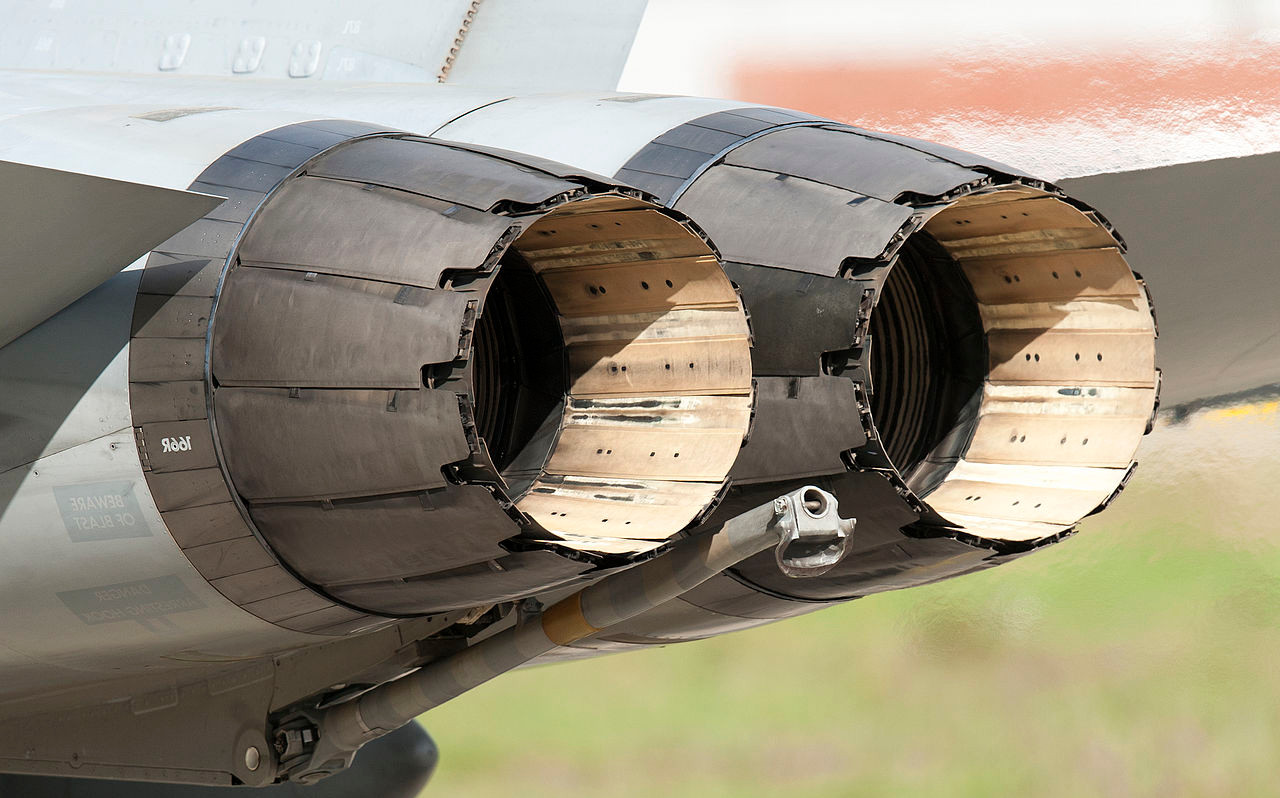
\includegraphics[width=8cm]{images/photo_tuyere.jpg}
			\end{center}
			\supercaption{Tuyères de deux GE F404.\\
			La géométrie de la tuyère, d’importance capitale en mécanique des fluides, n’est pas abordée dans ce document.}{\wcfile{1280px-Swiss_F-18_Hornet.jpg}{Photo} \ccbysa par \href{http ://www.flickr.com/people/39270009@N02}{Peng Chen}}
			\label{fig_illustration_tuyere1}
		\end{figure}

		\begin{figure}
			\begin{center}
				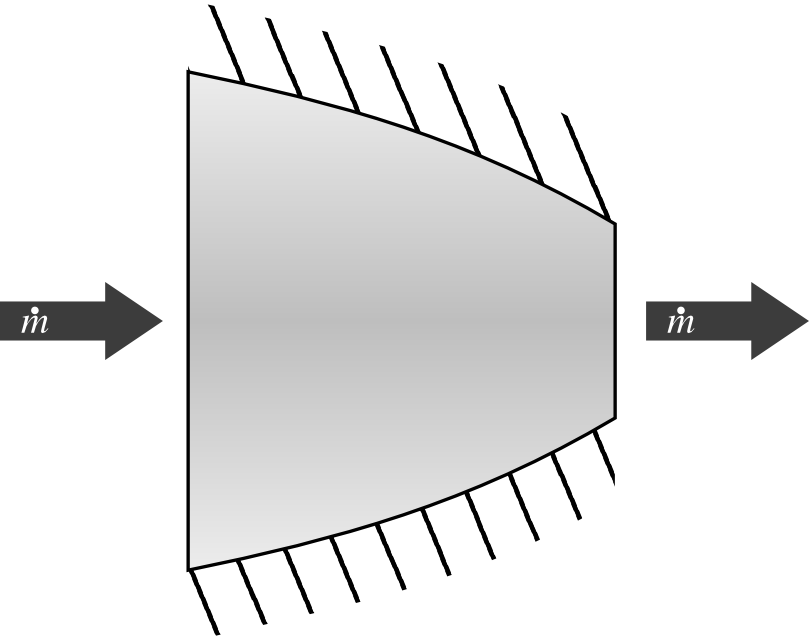
\includegraphics[width=5cm]{images/symbole_tuyere.png}
			\end{center}
			\caption{Représentation schématique d’une tuyère.}
			\label{fig_illustration_tuyere2}
		\end{figure}

		Un rapide rappel de l’équation énergétique en régime permanent, \textsc{sfee} (\ref{eq_petite_sfee_deltas_h}), nous permet de quantifier la vitesse finale des gaz en fonction de la différence de pression disponible :

		% \tag{\ref{eq_petite_sfee_deltas_h}}
		\begin{IEEEeqnarray}{rCl}
			q_{1 \to 2} + w_{1 \to 2} 		& = & \Delta h + \Delta e_{m}  		\\ 
			h_1 + \frac{1}{2} C_{\text{moy.}1}^2		& = & h_2 + \frac{1}{2} C_{\text{moy.}2}^2
		\end{IEEEeqnarray}

		Dans le cas d’une tuyère idéale, la détente est isentropique et nous pouvons relier les températures $T_1$ et $T_2$ tout comme au sein d’une turbine ou d’un compresseur, par les abominables relations \ref{eq_isentropique_horrible1} à \ref{eq_isentropique_horrible3}.

		Si les conditions fixent $h_1$ et $p_1$ {(sortie de turbine) ainsi que $p_2$ {(pression atmosphérique), on peut donc quantifier la variation de vitesse du gaz :
		\begin{equation}
			C_{\text{moy.}2}^2 - C_{\text{moy.}1}^2 	= 2 c_p (T_2 - T_1)
		\end{equation}

		Idéalement, la tuyère détend les gaz jusqu’à pression ambiante, et convertit toute la variation d’enthalpie des gaz en énergie cinétique. En pratique, bien sûr, une partie de cette énergie est convertie en chaleur par frottement. L’efficacité des tuyères est mesurée de façon similaire à celle des compresseurs et turbines, et n’est pas étudiée dans ce document.

		La conception des tuyères est bien plus complexe que cette section laisse paraître, surtout lorsque les composants avoisinent la vitesse du son. L’étudiant/e aurait tort de n’y voir qu’un simple «~tuyau thermodynamique~» même si c’est l’usage que nous en faisons ici.

		Notons pour finir que l’\vocab{entrée d’air} des moteurs aéronautiques joue souvent le rôle de diffuseur, c’est-à-dire l’inverse de la tuyère --\ elle ralentit l’air pour augmenter sa pression. Sur les moteurs supersoniques, un taux de compression de 2 est ainsi souvent atteint avant même l’entrée dans le compresseur, avec une augmentation correspondante de la température.




\section{Les configurations des turbomachines}



	\subsection{Intérêt des turbomachines}

		Les turbomachines, c’est-à-dire les moteurs fonctionnant avec une turbine (parfois simplement appelés «~turbines à gaz~»%
			\footnote{Cette appellation est particulièrement utilisée en anglais : «~\vocabe{gas turbine}~» est souvent synonyme de «~\vocabe{turbomachine}~».}%
		), présentent deux grands avantages par rapport à leurs homologues à pistons-cylindres :

		\begin{itemize}
			\item Le rapport puissance-poids des turbomachines est environ trois fois supérieur. Lorsque de grandes puissances sont requises avec contrainte d’espace ou de poids, les turbomachines sont incontournables ;
			\item Dans le cas de la propulsion aéronautique, le fluide moteur peut être utilisé comme médium de propulsion lui-même. Il suffit de laisser l’air sortir de la turbine avec une pression résiduelle et de le laisser se détendre dans une tuyère. On obtient alors une poussée par réaction (égale au débit de masse multiplié par sa vitesse) : c’est le principe du turboréacteur.
		\end{itemize}

		Parmi les inconvénients associés, on remarquera que l’efficacité et la réactivité des turbomachines chutent très rapidement à faible puissance. En effet, à charge partielle, le taux de compression et l’efficacité isentropique des turbines et compresseurs s’effondrent (pour des raisons qui seront étudiées en cours de mécanique des fluides). 

		Les turbomachines sont donc utilisées lorsque de hautes puissances sont requises de façon soutenue. Par exemple, le secteur automobile, où les variations de puissance sont nombreuses et doivent être actées instantanément, leur est inaccessible.



	\subsection{Le cœur du moteur, ou le «~générateur à gaz~»}

		Le cœur de tout moteur à turbine, souvent appelé \vocab{générateur à gaz}, ne comporte qu’un arbre et qu’une seule turbine (\cref{fig_générateur_gaz}). Cette section de machine n’a pas d’utilité en elle-même, mais l’air à sa sortie, dont la pression est plus haute que la pression d’entrée, peut être utilisé dans une multitude d’applications.

		\begin{figure}
			\begin{center}
				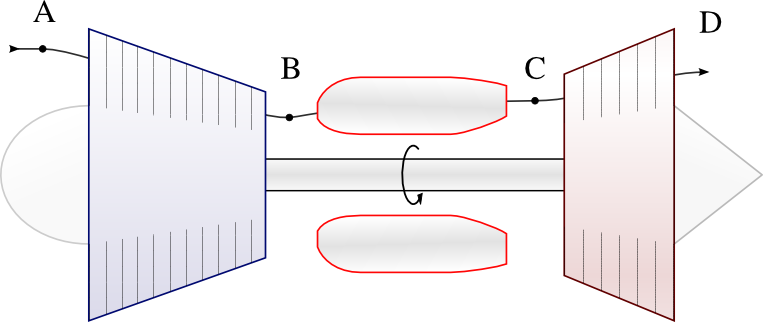
\includegraphics[scale=0.6]{images/circuit_generateur_gaz.png}\vspace{0.5cm}
				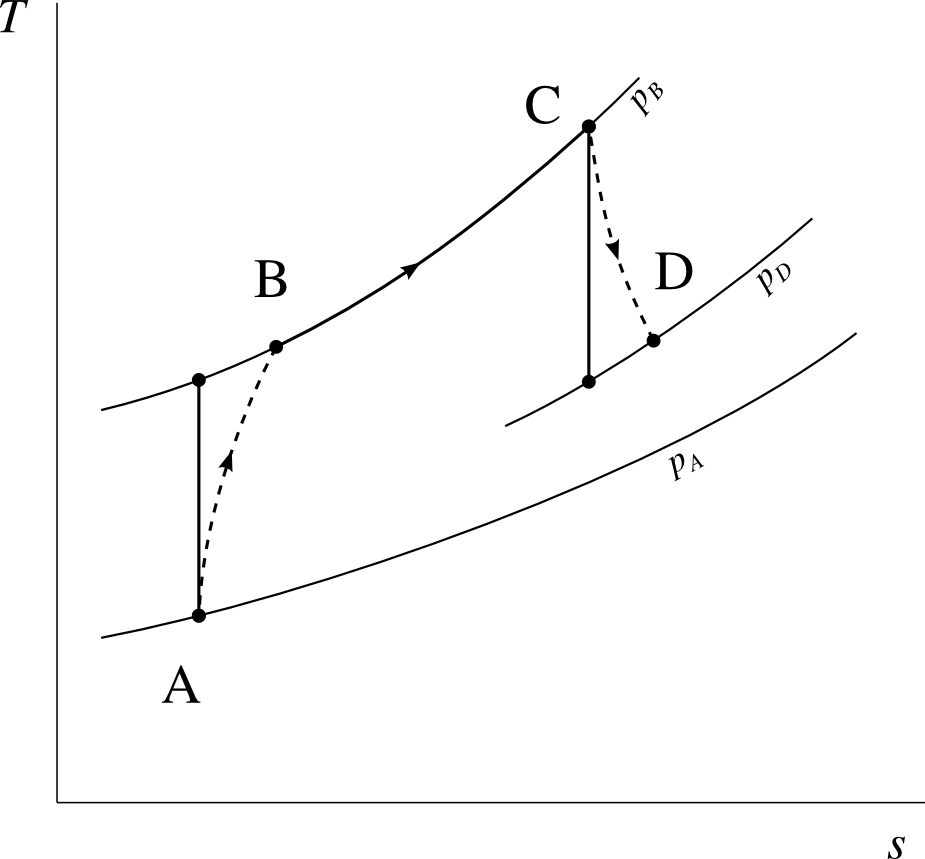
\includegraphics[scale=0.8]{images/ts_gp_generateur_gaz.png}
			\end{center}
			\supercaption{Cœur de turbomachine, ou «~générateur à gaz~» (schéma de fonctionnement et diagramme température-entropie).\\
			Cette installation n’a pas d’intérêt en elle-même mais a de nombreuses applications dérivées.}{\ccbysa \olivier}
			\label{fig_générateur_gaz}
		\end{figure}

		Dans cette configuration la turbine extrait exactement assez de puissance pour alimenter le compresseur. À sa sortie, l’air est encore comprimé et peut être exploité d’une multitude de façons.



	\subsection{Turboréacteur}

		Le \vocab{turboréacteur} (\cref{fig_turboréacteur}) est la première application qui ait été faite du moteur décrit plus haut. 

		À la sortie de la turbine, l’air est détendu dans une tuyère, ce qui l’accélère et fournit une poussée nette. C’est le fluide moteur lui-même qui est utilisé pour générer la poussée.

		\begin{figure}
		 	\begin{center}
				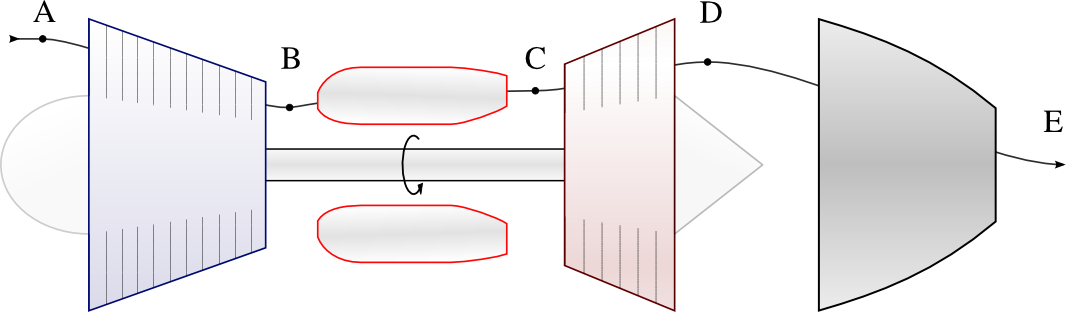
\includegraphics[scale=0.6]{images/circuit_turbojet.png}\vspace{0.5cm}
				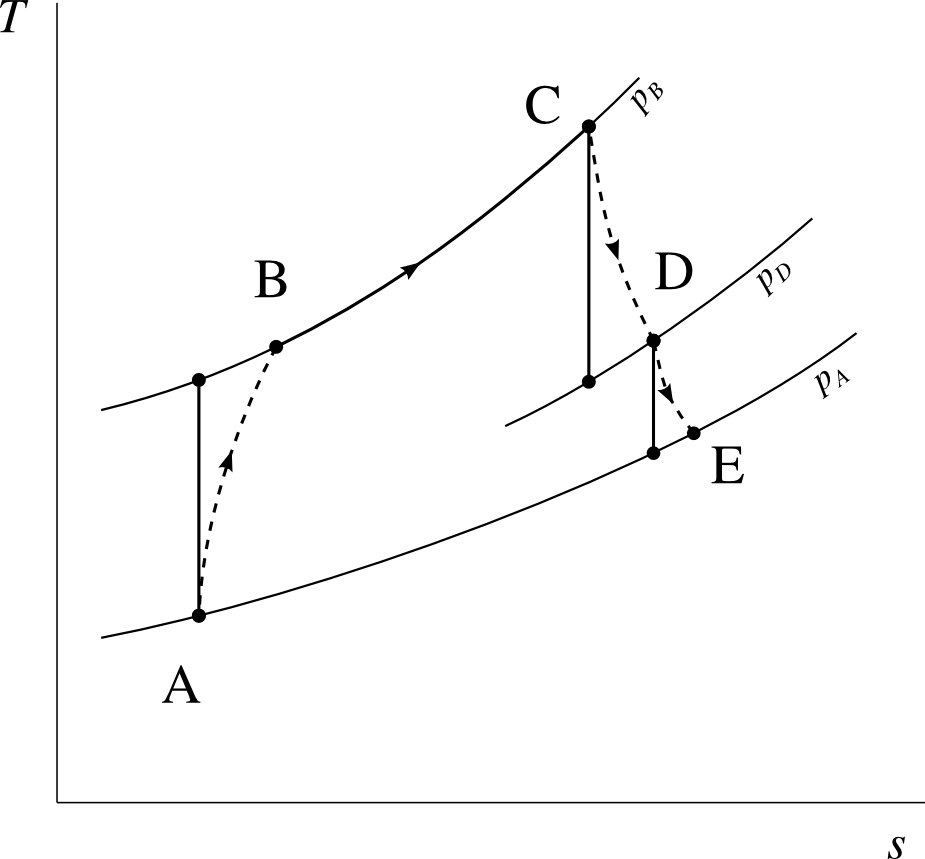
\includegraphics[scale=0.8]{images/ts_gp_turbojet.png}
			\end{center}
			\supercaption{Turboréacteur (schéma de principe et diagramme température-entropie).
			À la sortie de la turbine, l’air est encore pressurisé ; il est détendu dans une tuyère pour y être accéléré.}{\ccbysa \olivier}
			\label{fig_turboréacteur}
		\end{figure}

		Les turboréacteurs sont extrêmement compacts et utilisés principalement sur les appareils militaires.

		 

	\subsection{Turbopropulseur et turbomoteur}
	\label{ch_turboprop_turboshaft}

		Plutôt que d’utiliser une tuyère comme dans un turboréacteur, il est possible de poursuivre la détente dans la turbine jusqu’à la pression atmosphérique. La puissance fournie par la turbine est alors supérieure à la puissance consommée par le compresseur. 

		L’arbre moteur fournit alors du travail, que l’on peut utiliser pour alimenter une hélice (cas d’un \vocab{turbopropulseur}) ou un élément externe comme une génératrice ou une pompe (cas d’un \vocab{turbomoteur}), comme montré en \cref{fig_turbomoteur}.

		\begin{figure}
			\begin{center}
				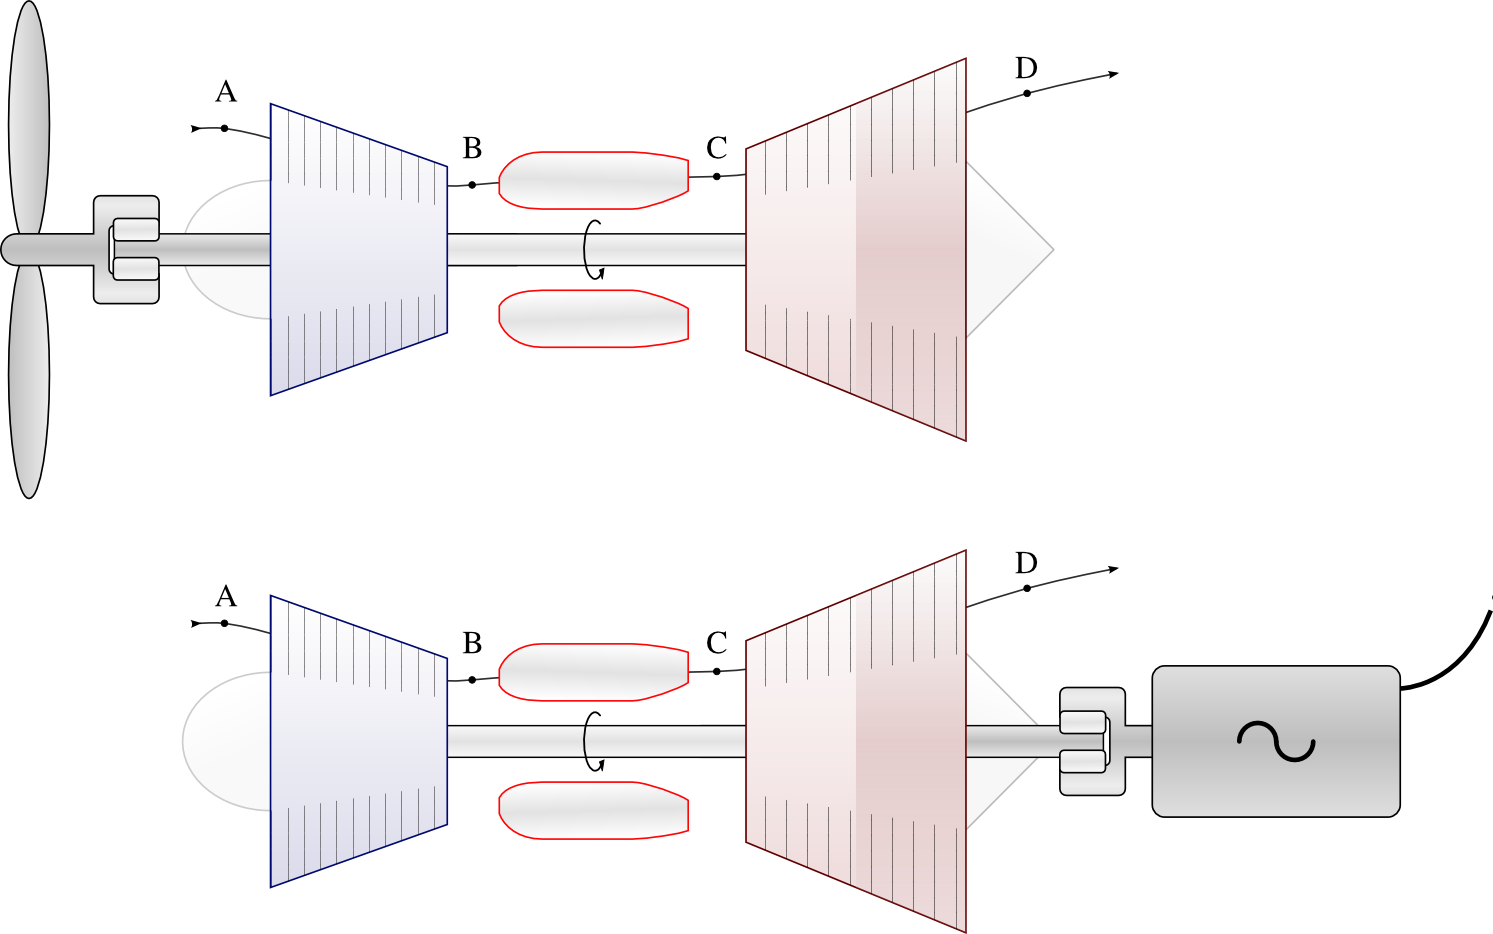
\includegraphics[scale=0.6]{images/circuit_turboprop_generateur.png}\vspace{0.5cm}
				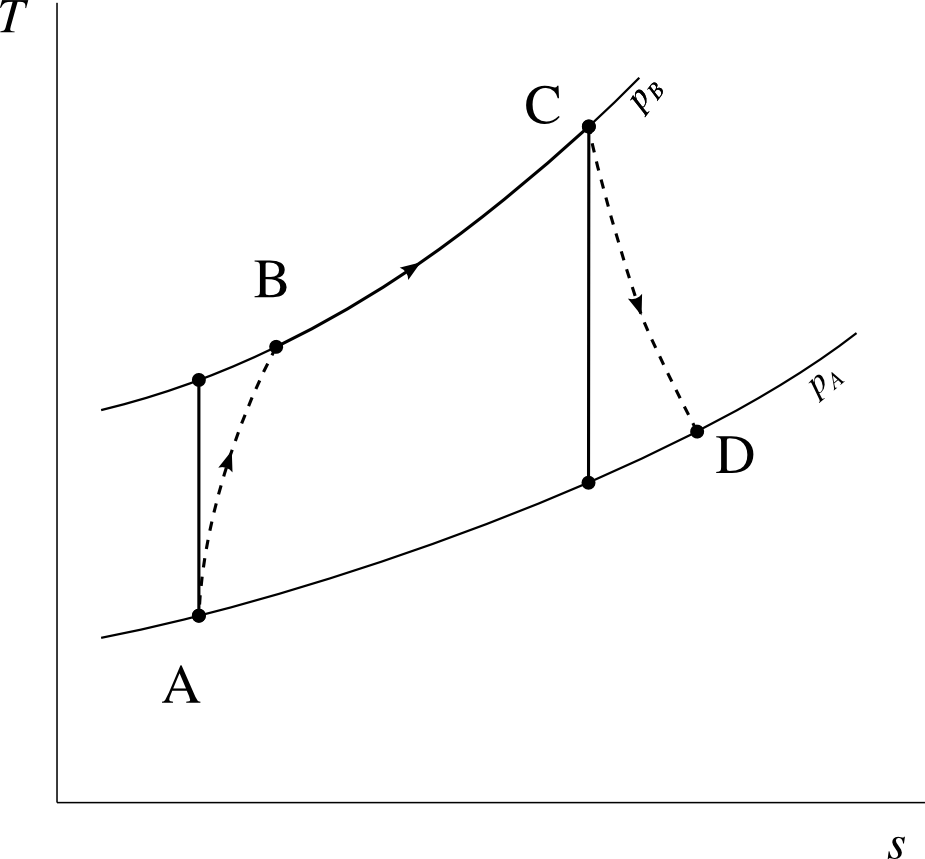
\includegraphics[scale=0.8]{images/ts_gp_turboprop_generateur.png}
			\end{center}
			\supercaption{Schémas de principe et diagramme température-entropie d’un turbopropulseur (haut) et d’un turbomoteur (bas). La puissance extraite de la turbine dépasse celle consommée par le compresseur, et est utilisée pour alimenter l’hélice ou bien une génératrice.}{\ccbysa \olivier}
			\label{fig_turbomoteur}
		\end{figure}

		L’alimentation d’une hélice de turbopropulseur, ou de la soufflante d’un turbofan, présente des avantages considérables en efficacité de propulsion que l’étudiant/e pourra étudier lors d’un cours de propulsion aéronautique. Les désavantages associés sont bien sûr l’encombrement et le poids : le diamètre des hélices et soufflantes dépasse souvent trois mètres, et elles imposent de grandes contraintes structurelles et mécaniques sur le moteur.

		Les turbomoteurs, quant à eux, ont de multiples applications (hélicoptères, navires militaires, générateurs électriques d’appoint, centrales génératrices à gaz…). Ils sont plus souvent déclinés dans les variantes détaillées plus bas.

		 

	\subsection{Turbofan}

		D’un point de vue thermodynamique, un \vocab{turbofan}\footnote{Un turbofan est parfois nommé \vocab{turboréacteur à soufflante} ou \vocab{à double flux}.} (\cref{fig_turbofan}), est équivalent à un turbopropulseur caréné, c’est-à-dire autour duquel on aurait placé un fuselage (nommé carène)\footnote{Le subtil effet d’une carène et la différence exacte entre turbofan et turbopropulseurs pourront être étudiés dans un cours de propulsion aéronautique.}. 
		
		\begin{figure}
			\begin{center}
				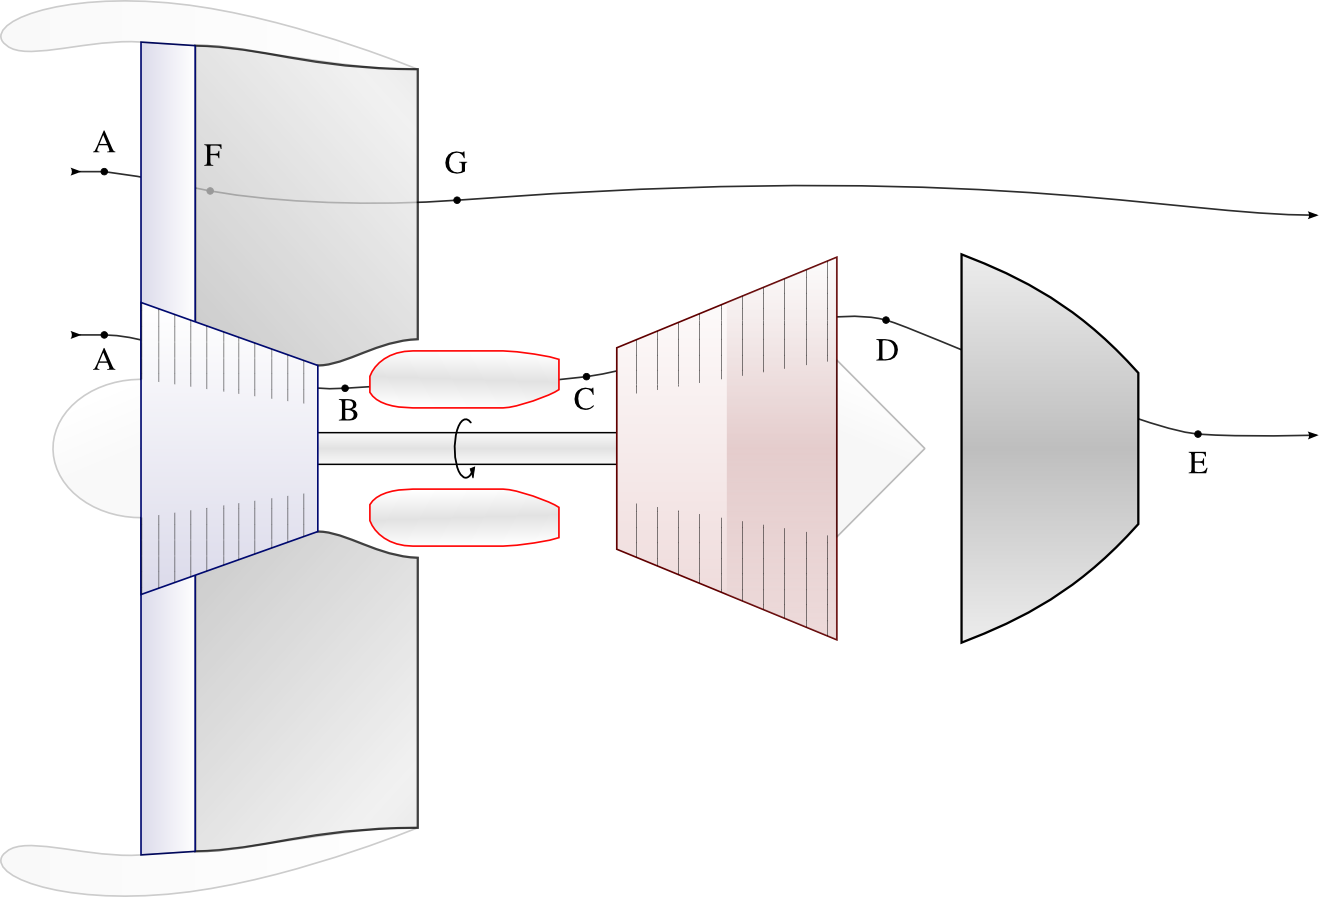
\includegraphics[scale=0.6]{images/circuit_turbofan.png}
			\end{center}
			\supercaption{Schéma de principe d’un turbofan. 
			Le circuit central du moteur ($\A \to E$) alimente mécaniquement la soufflante, qui permet au circuit externe ($\A \to G$) de fournir la majorité de la poussée.}{\ccbysa \olivier}
			\label{fig_turbofan}
		\end{figure}
		
		Il y a deux flux d’air séparés au sein d’un turbofan :

		\begin{itemize}
			\item le flux central, dit parfois «~flux chaud~», est le flux du moteur proprement dit. Après combustion, il traverse une turbine dont la puissance excède largement celle du compresseur. Cet excès de puissance est transmis à la soufflante ;
			\item le flux externe, dit parfois «~flux froid~», est faiblement compressé par la soufflante (ou «~fan~») et directement détendu dans la tuyère qui englobe le corps chaud du moteur. Il n’est jamais chauffé.\\
			C’est cet air «~froid~» qui fournit la plus grande part de la poussée\footnote{On montre que plus le rapport air froid / air chaud, (nommé \vocab{taux de dilution}) est grand, plus le moteur est efficace. Le taux de dilution des moteurs modernes avoisine \num{10}.}\nolinebreak.
		\end{itemize}
		 

	\subsection{Turbine libre et turbines multiples}

		En fonction des applications, plusieurs agencements de turbines et compresseurs peuvent être considérés.

		Avec une configuration à \vocab{turbine libre}\footnote{En anglais, \vocab{free turbine} ou \vocab{split-shaft system}}, la puissance mécanique fournie par le moteur est transmise par une turbine dédiée (\cref{fig_turbine_libre}). Cela permet de maintenir chacun des deux axes à des vitesses différentes.

		\begin{figure}
			\begin{center}
				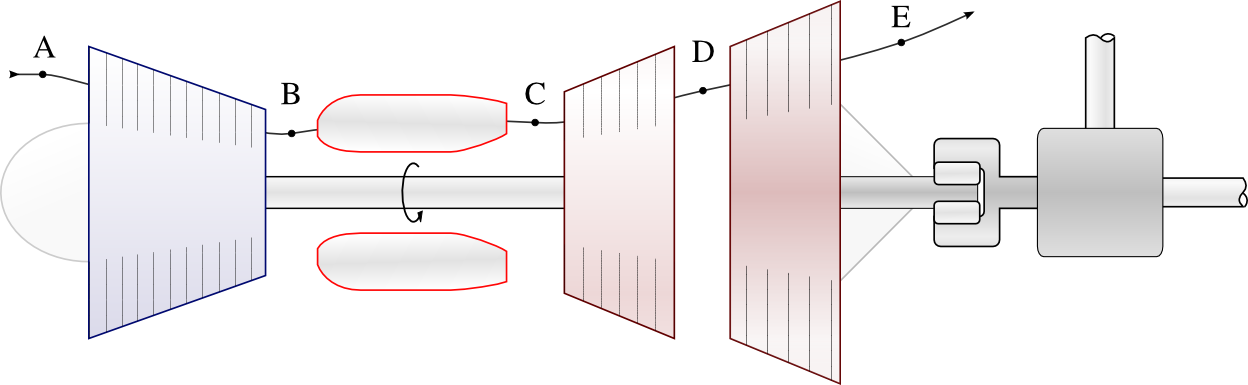
\includegraphics[scale=0.6]{images/circuit_turbine_libre.png}\vspace{0.5cm}
				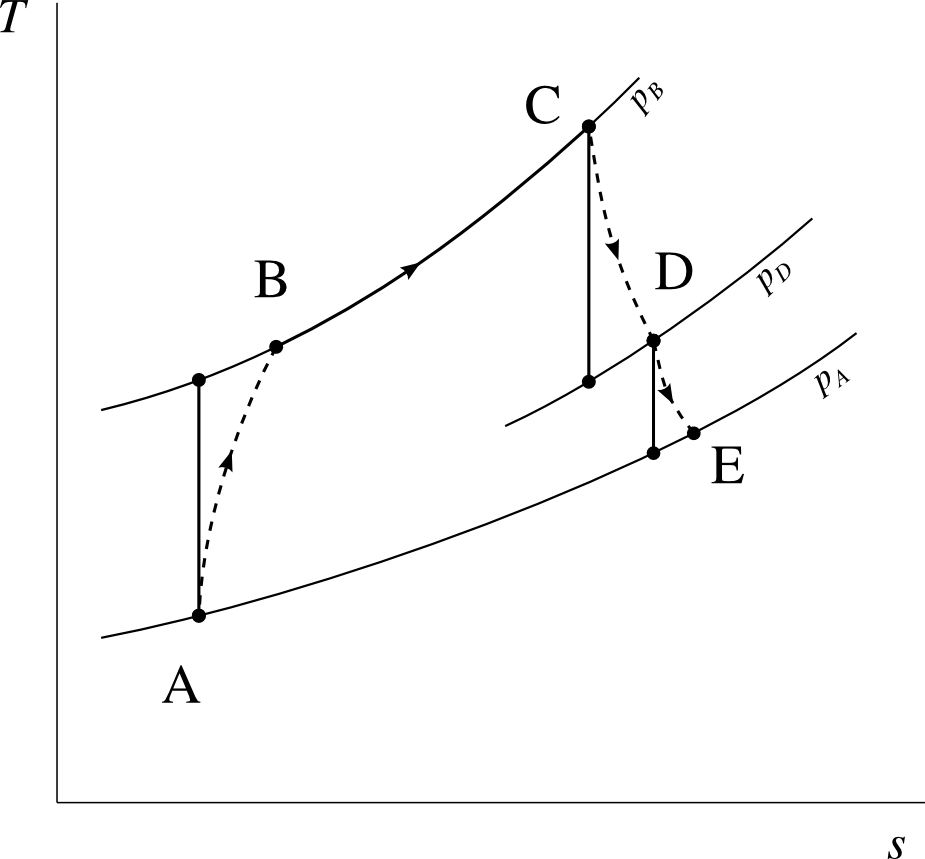
\includegraphics[scale=0.8]{images/ts_gp_turbine_libre.png}
			\end{center}
			\supercaption{Turbomoteur à turbine libre (schéma de principe et diagramme température-entropie).
			La puissance fournie par le moteur provient exclusivement de la turbine libre.}{\ccbysa \olivier}
			\label{fig_turbine_libre}
		\end{figure}

		La vitesse de l’axe turbine/compresseur n’étant pas contrainte par la charge imposée à l’axe libre, il peut évoluer à des vitesses plus proches de son point optimum, et accélérer plus aisément. Cet avantage compense la plus grande complexité mécanique lorsque les applications requièrent de grandes variations de puissance (en particulier la motorisation des hélicoptères).

		Avec une configuration à \vocab{axes multiples}\footnote{En anglais, \vocab{multiple-spool system} (notamment \textit{twin-} et \textit{triple-spool systems}).}, on divise compresseur et turbine en deux parties chacun, formant ainsi deux systèmes co-axiaux incorporés l’un dans l’autre (\cref{fig_axes_multiples}).

		\begin{figure}
			\begin{center}
				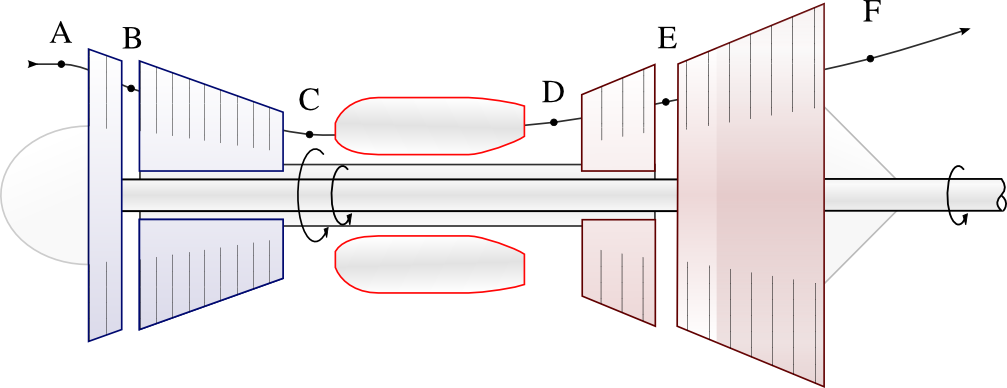
\includegraphics[scale=0.6]{images/circuit_twin_spool.png}\vspace{0.5cm}
				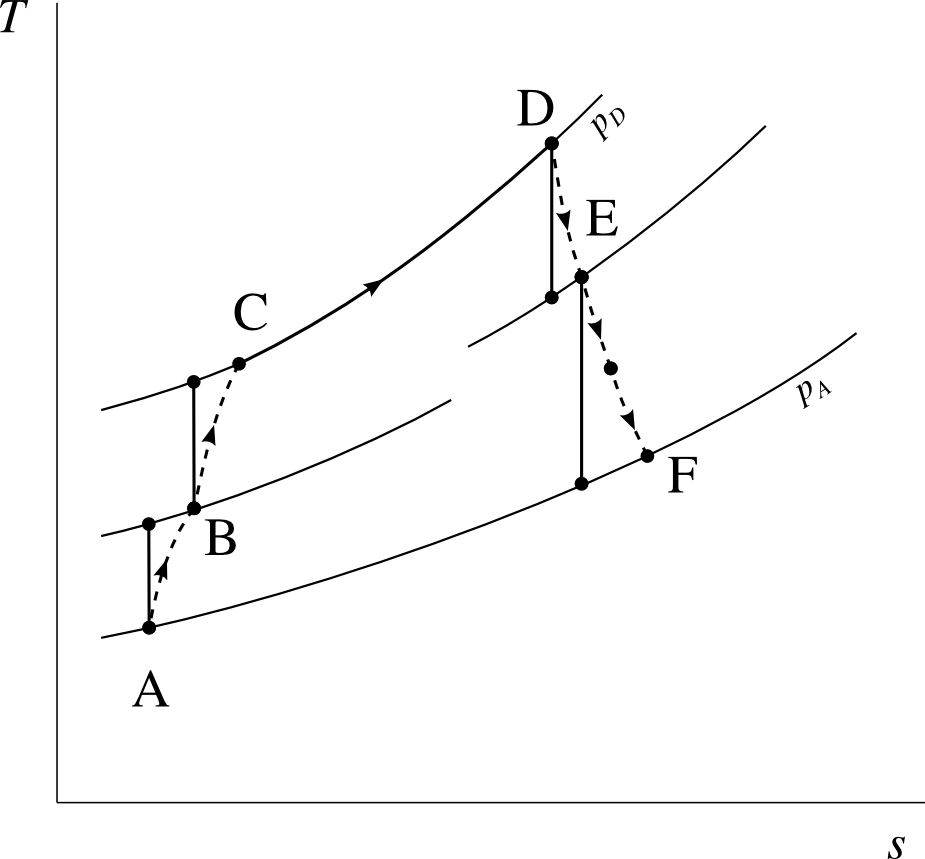
\includegraphics[scale=0.8]{images/ts_gp_twin_spool.png}
			\end{center}
			\supercaption{Turbomoteur à axes multiples (schéma de principe et diagramme température-entropie).
			Chaque axe tourne à une vitesse différente.}{\ccbysa \olivier}
			\label{fig_axes_multiples}
		\end{figure}

		C’est la turbine haute pression qui alimente le compresseur haute pression (axe à grande vitesse), et la turbine basse pression qui alimente le compresseur basse pression (axe à faible vitesse).

		L’objectif de l’agencement est le même que pour la turbine libre : permettre à chaque axe d’évoluer à sa vitesse propre. En effet, au fur et à mesure que la pression augmente dans le compresseur, la densité et la température augmentent. On peut alors faire évoluer les pales à plus grande vitesse et réduire ainsi leur taille.




\section{Modification des cycles des turbomachines}


	\subsection{Refroidissement intermédiaire et réchauffe}

		Pour les raisons citées en section \S\ref{ch_rapport_des_puissances} plus haut, il est souvent souhaitable d’aug\-menter le rapport des puissances, même au prix d’une baisse du rendement total.

		Pour réduire la puissance consommée par le compresseur, on a parfois recours au \vocab{refroidissement intermédiaire} (ou \vocab{intercooling}). La compression est interrompue, et l’air est refroidi avant de poursuivre la compression (\cref{fig_intercooling_réchauffe}).

		\begin{figure}
			\begin{center}
				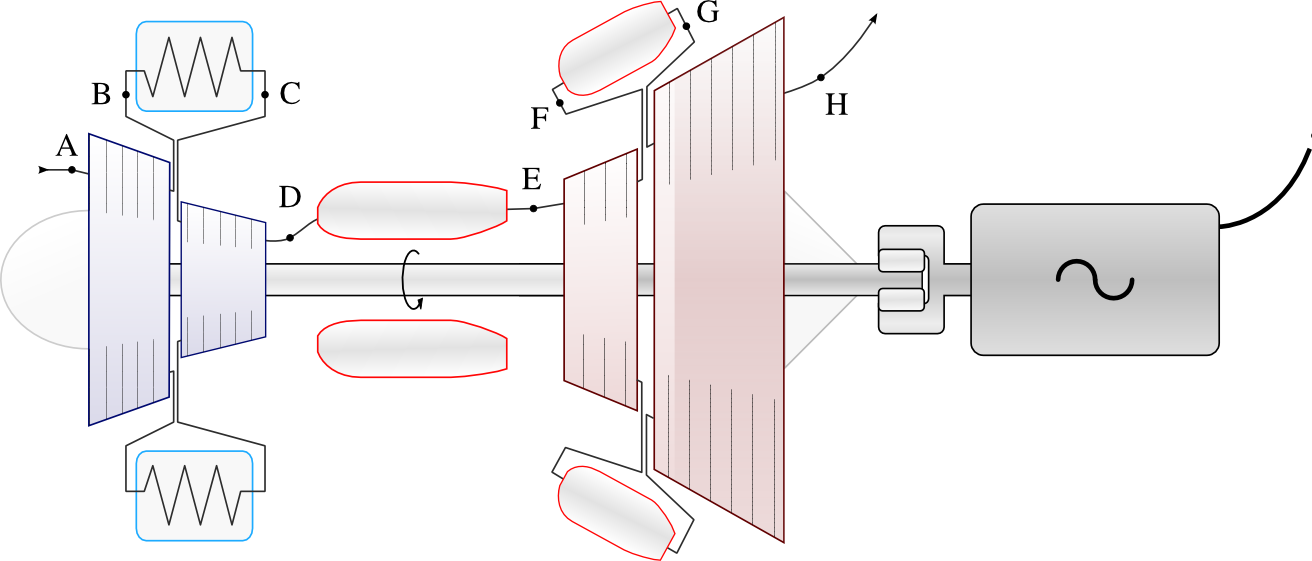
\includegraphics[scale=0.6]{images/circuit_intercooler_rechauffe.png}\vspace{1cm}
				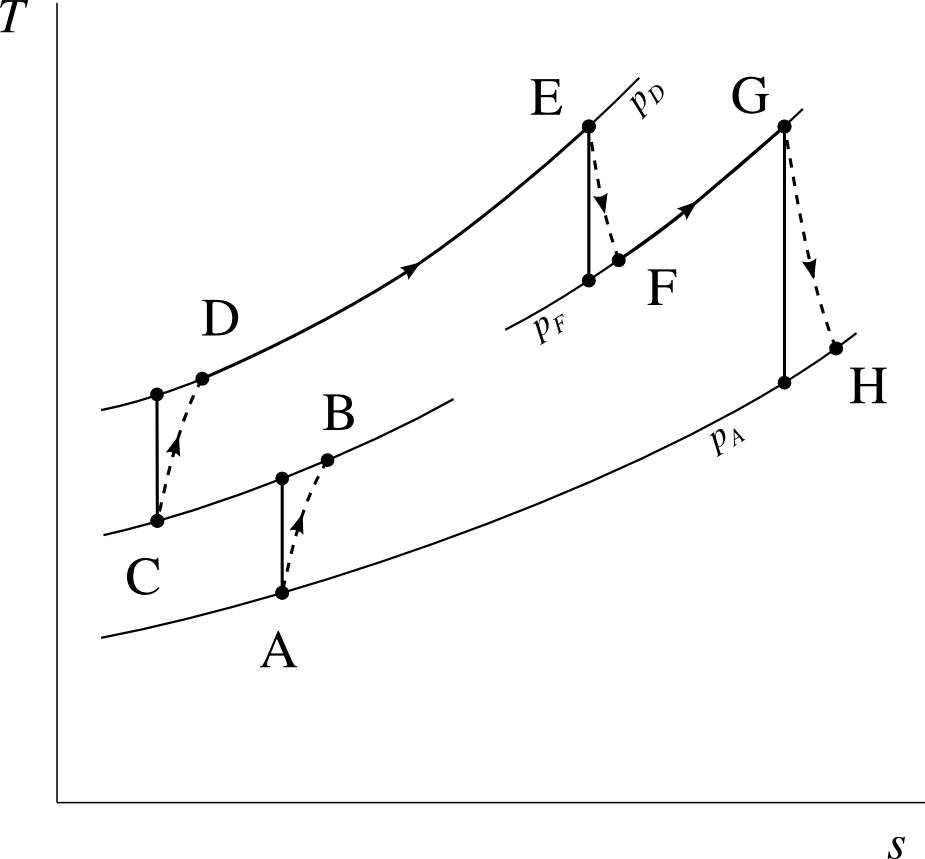
\includegraphics[scale=0.8]{images/ts_gp_intercooler_rechauffe.png}
			\end{center}
			\supercaption{Turbomoteur générateur avec refroidisseur et réchauffe (schéma de principe et diagramme température-entropie)\\
			Le refroidisseur («~\vocab{intercooler}~») refroidit l’air au milieu de sa compression ; tandis que la deuxième chambre de combustion le réchauffe au milieu de la détente. Les deux modifications sont indépendantes l’une de l’autre et peuvent être installées séparément.}{\ccbysa \olivier}
			\label{fig_intercooling_réchauffe}
		\end{figure}

		La compression d’un gaz entre deux pressions données impose un \emph{rapport} entre les températures initiale et finale (\ref{eq_isentropique_horrible1}). Par contre, la puissance demandée pour compresser un gaz entre ces deux pressions dépend de la \emph{différence} entre ces deux températures (\ref{eq_puissance_compresseur}). Ainsi, plus la température de départ est faible, et plus la puissance nécessaire pour atteindre une pression donnée sera faible.

		Dans la même optique, on peut augmenter la puissance spécifique fournie par la turbine en procédant au réchauffement des gaz avant la fin de la détente : c’est la \vocab{réchauffe}. Le principe et le procédé sont identiques à la resurchauffe des centrales à vapeur (\S\ref{ch_resurchauffe}).

		Il n’aura pas échappé à l’étudiant/e que le rendement est inévitablement réduit par l’utilisation du refroidissement intermédiaire. La chambre de combustion doit en effet fournir plus de chaleur, à température moyenne plus basse. Cette réduction du rendement fera l’objet d’un compromis avec la réduction de la taille du compresseur (usuellement la pièce la plus volumineuse d’un moteur) et l’augmentation de la puissance spécifique. Refroidissement intermédiaire et réchauffe sont caractéristiques des installations où le rapport puissance/encombrement doit être maximisé.

		Pour réduire la perte de rendement, il est parfois possible, dans les moteurs au sol, de récupérer de la chaleur des gaz d’échappement pour réchauffer l’air à la sortie du compresseur, et ainsi soulager la chambre de combustion à moindres frais énergétiques. L’échangeur de chaleur est parfois appelé \vocab{économiseur} (\cref{fig_intercooler_echangeur}) ; il est laissé à l’étudiant/e le loisir de retracer le cycle suivi sur un diagramme température-entropie et de retrouver les conditions nécessaires à son fonctionnement.
		
		\begin{figure}
			\begin{center}
				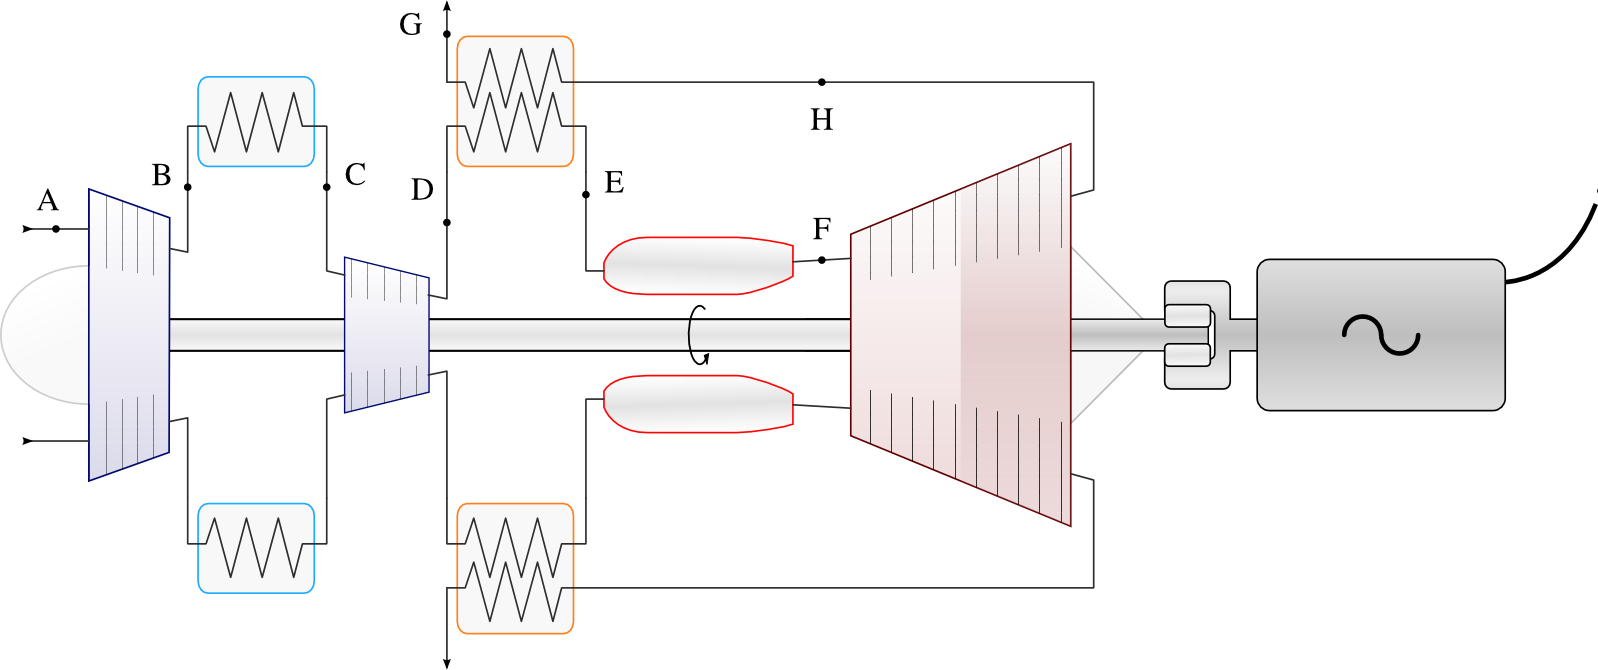
\includegraphics[scale=0.6]{images/circuit_intercooler_echangeur.png}
			\end{center}
			\supercaption{Turbomoteur générateur avec refroidisseur et échangeur économiseur (schéma de principe)\\
			Les gaz d’échappement sont redirigés vers l’intérieur du moteur pour fournir de la chaleur aux gaz à l’entrée de la chambre de combustion. Il est laissé à l’étudiant/e le soin de déterminer les limites du procédé.}{\ccbysa \olivier}
			\label{fig_intercooler_echangeur}
		\end{figure}

	\subsection{Postcombustion}
	\label{ch_postcombustion}

		La \vocab{postcombustion}\footnote{En anglais, \vocab{afterburning}.} est l’ajout d’une seconde phase de combustion dans un turboréacteur, après la turbine et avant l’entrée dans la tuyère (\cref{fig_postcombustion}). Le principe est exactement le même que celui de la réchauffe : augmenter la poussée spécifique de la machine (au détriment de son rendement).

		\begin{figure}
			\begin{center}
				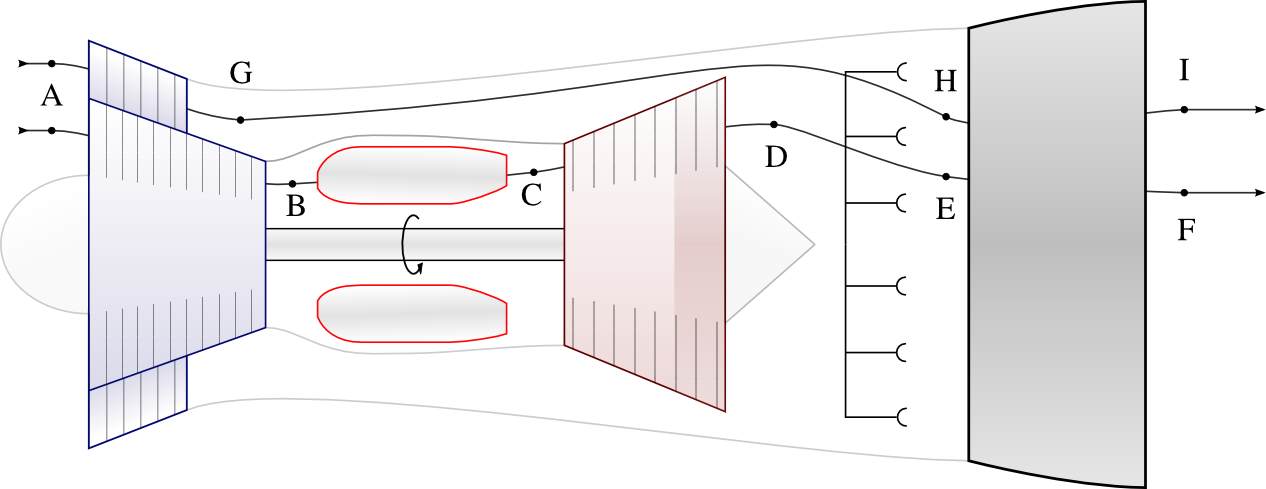
\includegraphics[scale=0.6]{images/circuit_postcombustion.png}\vspace{0.5cm}
				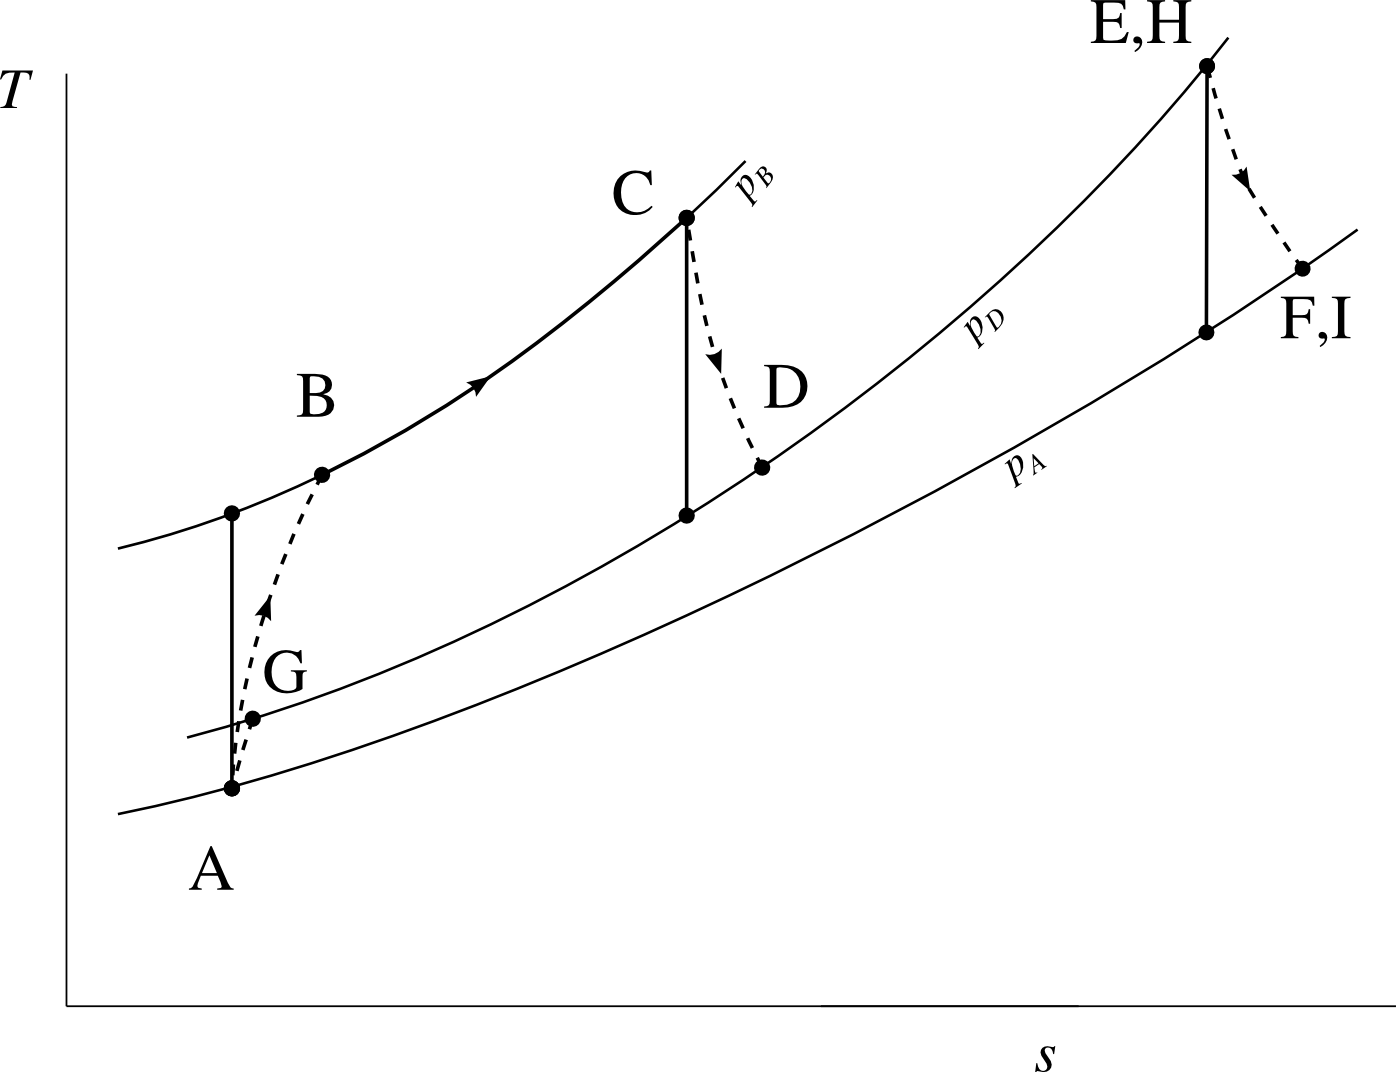
\includegraphics[scale=0.8]{images/ts_gp_postcombustion.png}
			\end{center}
			\supercaption{Postcombustion sur un turboréacteur double-flux (schéma de principe et diagramme température-entropie).\\
			Les états $E$ et $H$ ne sont en pratique pas nécessairement confondus.}{\ccbysa \olivier}
			\label{fig_postcombustion}
		\end{figure}

		Tout comme la réchauffe, la postcombustion modifie les propriétés (le volume spécifique en particulier) de l’air et impose un redimensionnement des pièces en aval. La géométrie de la tuyère est ainsi modifiée en fonction de l’activation ou non de la postcombustion.

		L’ajout d’un système de postcombustion à un turboréacteur ne nécessite que l'in\-stal\-la\-tion de brûleurs ainsi que d’un système de variation de la géométrie sur la tuyère. L’augmentation du poids engendrée est faible au regard de l’augmentation de la puissance.

		La perte outrageante de rendement engendrée par l’utilisation de la postcombustion, ainsi que les niveaux fracassants de bruit et de pollution qu’elle engendre, la limitent au seul domaine militaire (sur les avions de combat en particulier).

		 

	\subsection{Refroidissement de la turbine}

		L’intérêt présenté par l’obtention de hautes températures dans la chambre de combustion pousse les constructeurs à développer toute une série de technologies pour maximiser la température en sortie de chambre de combustion (\textsc{tet}, pour \vocab{Turbine Entry Temperature}).

		Le principal stratagème employé est de refroidir la turbine avec de l’air prélevé sur le compresseur (\cref{fig_refroidissement_turbine}). L’air prélevé est conduit à l’intérieur des pales de la turbine et permet d’élever la température de combustion sans risquer d’endommager les pales.

		\begin{figure}
			\begin{center}
				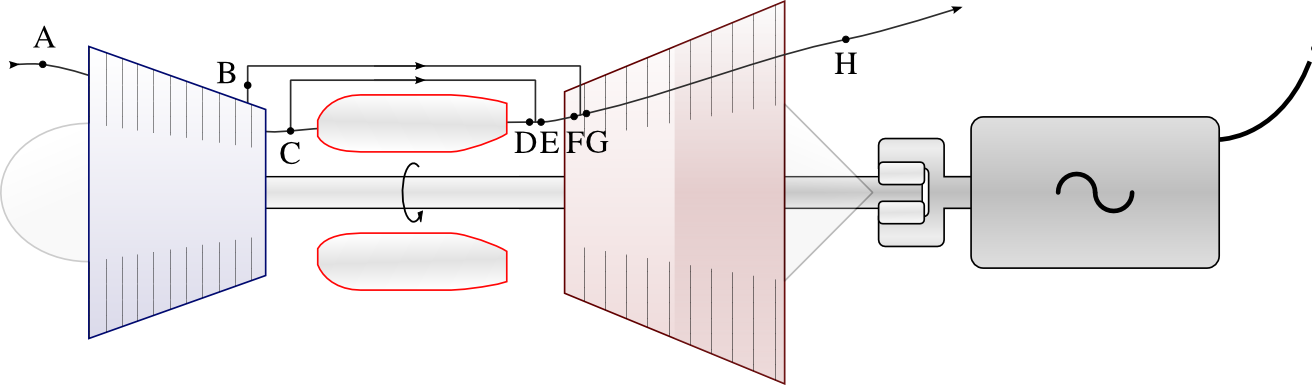
\includegraphics[scale=0.6]{images/circuit_refroidissement_turbine.png}\vspace{0.5cm}
				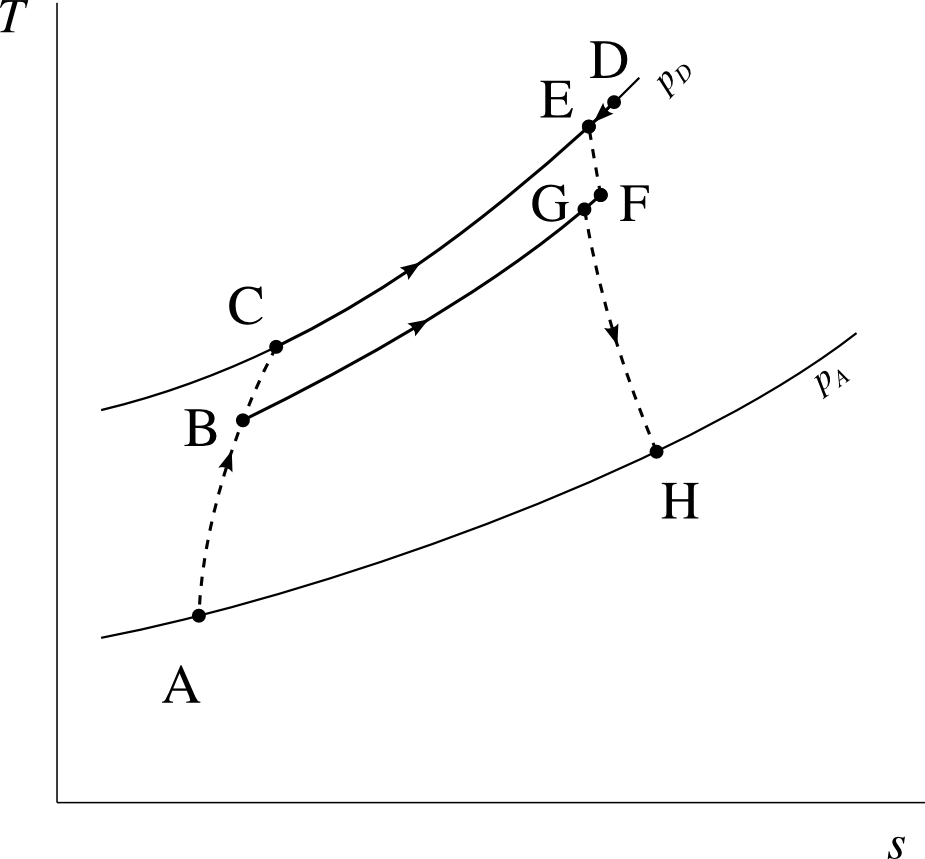
\includegraphics[scale=0.8]{images/ts_gp_refroidissement_turbine.png}
			\end{center}
			\caption{Refroidissement de la turbine à l’aide d’air prélevé sur le compresseur (schéma de principe et diagramme température-entropie).
			Cet air, à température modérée, contourne la chambre de combustion et n’entre jamais en contact avec le carburant. Ici le moteur représenté est un turbomoteur, mais le refroidissement turbine est utilisable sur toute configuration.}
			\label{fig_refroidissement_turbine}
		\end{figure}


		Les systèmes de refroidissement les plus efficaces et les plus avancés enrobent l’ex\-térieur des pales de turbine avec une couche d’air plus froid, tiré du compresseur. La température \textsc{tet} peut ainsi dépasser la température de fonte des pales de plus d’une centaine de degrés Celsius !

		Le refroidissement de la turbine a un coût conséquent. 

		D’une part, dans un moteur réel, la détente de l’air de refroidissement dans la turbine fournit moins d’énergie que n’en consomme sa compression dans le compresseur\footnote{Dans le cas limite où la compression et la détente sont isentropiques, ce coût énergétique est nul.}\nolinebreak.
			La circulation de cet air est donc une charge énergétique qui doit être compensée par l’augmentation de l’efficacité qu’elle engendre.

		D’autre part, le compresseur et la turbine doivent être sur-dimensionnés pour admettre un débit d’air plus grand, avec les conséquences décrites en début de chapitre.

		Le refroidissement des turbines est un axe majeur de recherche en propulsion aéronautique. Il faut maîtriser de nombreux domaines (matériaux, mécanique des fluides, agencement mécanique, chimie de combustion) pour remplir ces objectifs de nature thermodynamique.


		\begin{landscape}

		\begin{figure}
			\begin{center}\vspace{-3cm}
				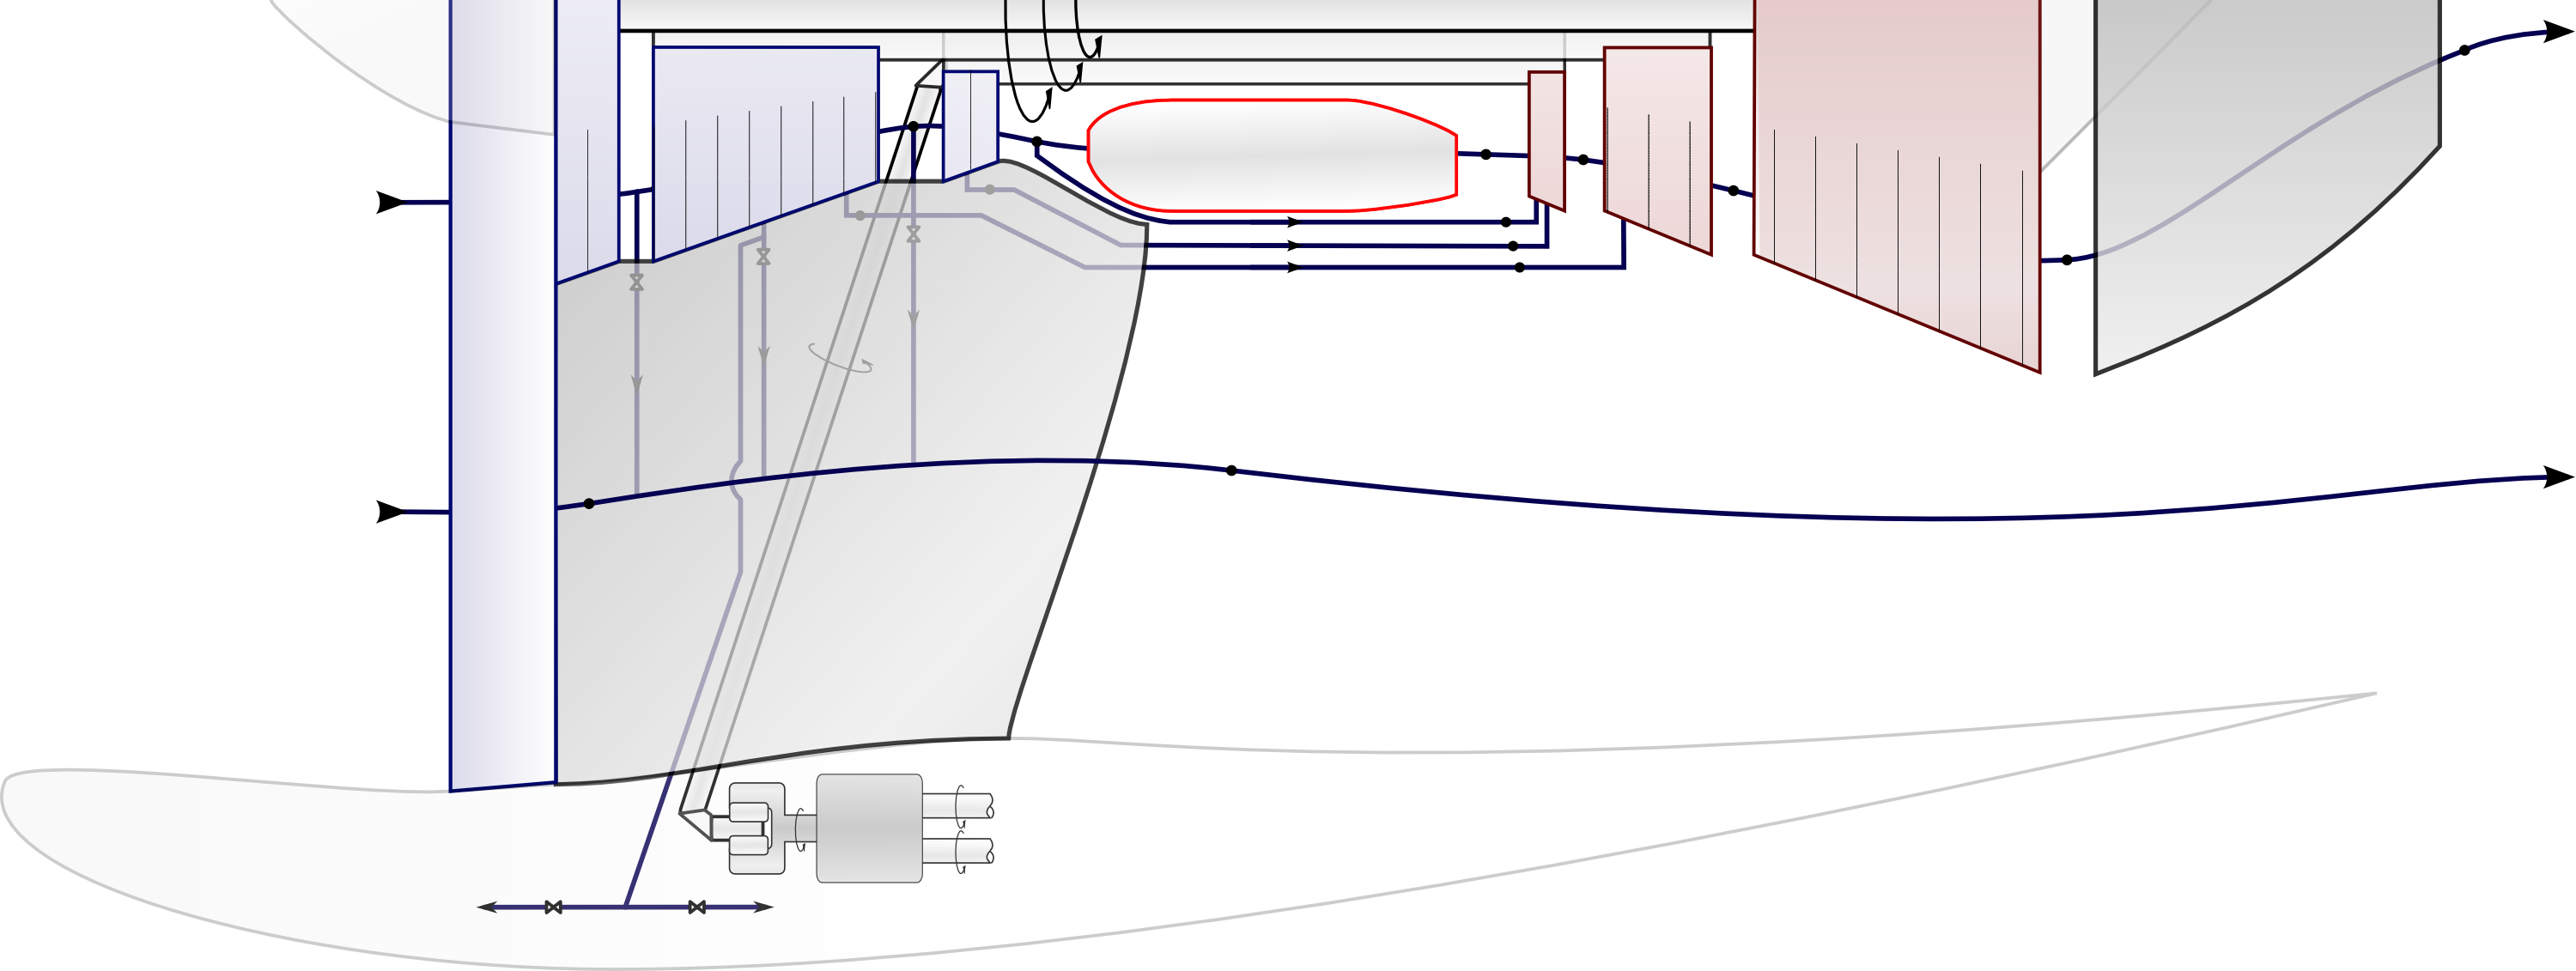
\includegraphics[width=19cm]{images/circuit_turbofan_complet.png}
			\end{center}
			\supercaption{Schéma du circuit thermodynamique d’un turbofan moderne.
			L’installation combine axes multiples, extractions de puissance mécanique et pneumatique, prélèvements de refroidissement turbine, et deux flux d’air principaux (il est laissé encore à l’étudiant/e le loisir de tracer le cycle sur un diagramme température-entropie).
			Sur les bimoteurs qualifiés \textsc{etops}, chaque moteur doit pouvoir assurer seul le vol de l’appareil et l’alimentation de nombreux systèmes (pressurisation, chauffage, génération électrique et pneumatique) pendant plusieurs heures avec une fiabilité démontrée.}{\ccbysa \olivier}
		\end{figure}

		\end{landscape}
